% #############################################################################
% This is Chapter 5
% !TEX root = main.tex
% #############################################################################
% Change the Name of the Chapter i the following line
\fancychapter{Assessment \& Implications}
\clearpage
% The following line allows to ref this chapter
\label{chap:chap005}

\vspace{0.05mm}

\noindent
{\it This Chapter~\ref{chap:chap005} was published in two top (Q1 in 2021 and 2022, respectively) ranked journals:}

\vspace{0.05mm}

\begin{itemize}
\item {\bf Francisco Maria Calisto}, Carlos Santiago, Nuno J. Nunes, Jacinto C. Nascimento, Introduction of Human-Centric AI Assistant to Aid Radiologists for Multimodal Breast Image Classification, International Journal of Human-Computer Studies, Volume 150, 2021, 102607, ISSN 1071-5819. DOI: \href{https://doi.org/10.1016/j.ijhcs.2021.102607}{doi.org/10.1016/j.ijhcs.2021.102607}
\item {\bf Francisco Maria Calisto}, Carlos Santiago, Nuno J. Nunes, Jacinto C. Nascimento, BreastScreening-AI: Evaluating Medical Intelligent Agents for Human-AI Interactions, Artificial Intelligence in Medicine, Volume 127, 2022, 102285, ISSN 0933-3657, DOI: \href{https://doi.org/10.1016/j.artmed.2022.102285}{doi.org/10.1016/j.artmed.2022.102285}
\end{itemize}

For this thesis, the main goal is to understand how the implemented \ac{DL} methods (Appendix~\ref{chap:app004}) can be integrated within an intelligent agent.
Moreover, it is essential to understand how the intelligent agent(s) can better communicate with clinicians as a second reader.
In this chapter, we take an \ac{HCI} perspective on the implications of \ac{AI} techniques~\cite{CALISTO2022102285} across the assessment of medical imaging~\cite{CALISTO2021102607}, focusing on workflow efficiency and quality, preventing medical errors and variability of diagnosis in breast cancer.

\section{Motivation}
\label{sec:chap005001}

The combination of \ac{AI} and medical imaging, known as ``radiomics''~\cite{Lambin2017}, has the potential to revolutionize radiology by automating the analysis of large amounts of data and extracting meaningful features to support diagnosis and clinical decision-making~\cite{Ruddle:2016:DEI:2872314.2834117}.
However, while modern assistant technologies such as \ac{DL} methods show promising accuracy (Section~\ref{sec:app003001}), the probabilistic nature of their algorithms can lead to mistrust and abandonment by clinicians who do not expect their clinical systems to behave inconsistently and imperfectly~\cite{Kocielnik:2019:YAI:3290605.3300641}.
Therefore, evaluating the acceptance and usability of \ac{AI}-based clinical systems was crucial to ensure successful adoption (Chapter~\ref{chap:chap004}) in real-world clinical setups.

Deficiencies in experimental and analytic designs have been identified in some studies~\cite{Sultanum:2018:MTP:3173574.3173996}.
However, these studies fail to include a more holistic understanding of the clinical context.
Another important consideration on using \ac{AI} in real-world clinical settings is the trust and usability of interactive assistance techniques~\cite{Cadario2021}.
While much work has focused on improving the accuracy of \ac{AI} algorithms, comparatively less work has been done to improve trust and usability~\cite{CALISTO2021102607}.
Thus, our research aims to answer high-level questions about how radiologists accept and interact with AI-assisted systems, how receptive they are to their introduction, and how they are affected by \ac{AI} assistance in different clinical contexts~\cite{CALISTO2022102285, CALISTO2021102607}.
For that, we propose an \ac{AI}-assisted approach, which integrates \ac{DL} techniques with a real clinical workflow for a multimodal medical imaging diagnosis~\cite{10.1145/3399715.3399744}.
Our proposed approach aims to improve diagnosis accuracy and reduce cognitive workload.
We also consider the importance of providing reasons for \ac{AI} recommendations to foster model transparency and user trust.

\subsection{Contributions}
\label{sec:chap005001001}

We created our proposed technique, based on the following contributions:
(1) exploring the power of explanations and the users' need for control on the introduction of \ac{AI} methods among medical imaging diagnosis; and
(2) studying the \ac{AI} impact on the radiologists' {\it behaviour} in professional practice.
We did that to achieve higher user expectations of the system capabilities, addressing potential gaps.
Although efforts have been dedicated to enhancing the precision of \ac{AI} algorithms, there has been relatively less emphasis on enhancing trust and usability of interactive assistance techniques.
Therefore, we ask several high-level questions, namely:
i) how they {\it accept} and {\it interact} with these systems;
ii) how {\it receptive} are the clinicians to the introduction of \ac{AI} assistance;
iii) how clinicians are {\it affected} by the \ac{AI} assistance in different clinical contexts.
This chapter contributes broadly to the literature in \ac{HCI} and \ac{AI} by examining what radiologists need when using \ac{AI}-powered image diagnostic, the practices they adopt while using these tools, and how they affect end-user attitudes towards the underlying \ac{AI} algorithms.

\subsection{Research Questions}
\label{sec:chap005001002}

A vital component of this dissertation thesis was to access many clinical settings and radiologists.
In this thesis, the work has established the foundations of its research via a human-centered design process and following the literature guidelines (Section~\ref{sec:app003002} of Appendix~\ref{chap:app003}) for \ac{HAII}~\cite{10.1145/3313831.3376718, 10.1145/3290605.3300233, 10.1145/3290605.3300234, Kocielnik:2019:YAI:3290605.3300641}, including:
i) findings from a user study in nine clinical institutions, encompassing {\it in-situ} observations and interviews, as well as grounded by related work; which informed
ii) a list of design recommendations for medical imaging systems, including temporal awareness, image processing, multimodality, trust, acceptance, and usage; leading to
iii) findings from an evaluation study of {\it BreastScreening-AI}, a proof-of-concept prototype that was developed to support the clinical translation of {\it radiomics}, validated by 45 physicians; and finally
iv) evidence from the impact of multimodality and \ac{AI}-assisted strategy in diagnosing breast cancer patients and severity classification of lesions.

\vspace{2.50mm}

\noindent
By focusing on the integration of multimodality and \ac{AI} techniques in {\it BreastScreening-AI} and clinical workflows, we formulated the following three research questions:

\vspace{0.05mm}

%%%%%%%%%%%%%%%%%%%%%%%%%%%%%%%%%%%%%%%%%%%%%%%%%%
\begin{enumerate}
\item {\bf RQ5.1.} What is the impact on clinicians' satisfaction and acceptance of \ac{AI} assistance with applied design interventions in radiology?
\item {\bf RQ5.2.} How can we improve clinicians' understanding and trust in \ac{AI} recommendations using design techniques to increase the explainability power of the system?
\item {\bf RQ5.3.} What is the impact of \ac{AI} assistance on the medical workflow, including accuracy, time performance, and variability in patient classification?
\end{enumerate}
%%%%%%%%%%%%%%%%%%%%%%%%%%%%%%%%%%%%%%%%%%%%%%%%%%

\section{Background}
\label{sec:chap005002}

In this section, two areas motivate our research work:
a) related works designing autonomous systems ({\it e.g.}, {\it radiomics}, \acp{CADe}, \acp{CADx}, \acp{CDSSe}) for the clinical workflow, while providing an assisted medical imaging analysis; and
b) the theories of \ac{HAII} collaboration while covering users' expectations and potential gaps.
The section begins by outlining the role of design for the clinical workflow and how it is currently handled in various steps of the \ac{DL} pipeline (Figure~\ref{fig:fig027}) and {\it radiomics} stages, including image segmentation, feature extraction, and image classification.
Then, the section introduces the reader to existing \ac{HAII} techniques to facilitate the integration of those intelligent agents into the framework.

\subsection{Clinical Workflow Design}
\label{sec:chap005002001}

In modern healthcare, medical images play a crucial role in supporting decision-making for diagnosis, predictions, and treatment planning~\cite{liang2019deep}.
Accurate lesion detection and segmentation are often mandatory for image analysis and {\it radiomics}, where numerous methods have been proposed to automatically perform these tasks~\cite{litjens2017survey}.
In the field of breast cancer, medical imaging systems allow clinicians to diagnose several modalities from the retrieval of medical imaging data~\cite{seifabadi2019correlation}.
To enhance clinical workflows, a wide range of \acp{CDSSe} are designed, including those that provide potential information for medical decision-making and those that make diagnostic decisions~\cite{10.1145/3290605.3300234, GU2020101858}.
However, experts may resist using a system if it does not capture the nuances of their mental models or provides relevant context~\cite{yang2016investigating}.
Conversely, clinicians are known to resist changes and new tools~\cite{10.1145/3132272.3134111}, an issue that has an impact in their workflow.
In our research, we take a human-centered approach to understanding various design aspects and expectations of a medical imaging \ac{CDSSe} that is integrated into a real radiology workflow.
To accomplish this, we use methods such as bringing focus groups, workshops, observations, and interviews from the literature~\cite{Lim:2019:DDI:3319806.3301427} into our user research activities (Section~\ref{sec:chap005003001}).
By doing so, we aim to understand better how the system can be designed to meet the needs and expectations of its users (Section~\ref{sec:app003004007} of Appendix~\ref{chap:app003}), including radiologists and other medical professionals who work with the system on a regular basis.
In particular, our work demonstrates how an interactive \ac{AI} can directly address the above-mentioned challenges during medical imaging diagnosis.

The field of \ac{AI} is providing several \ac{DL} work models to assist clinical practitioners with appropriate knowledge~\cite{9540298, 9730804}.
However, the literature does not typically address the effectiveness of clinical \ac{AI} solutions from the perspective of human users~\cite{CALISTO2021102607}.
The work of Xie et al.~\cite{10.1145/3313831.3376807} has established the importance of providing reasons for the design of \ac{AI} recommendations to foster model transparency and user trust within these clinical workflows.
This work stressed that clinical systems should be designed based on the user needs of clinical practitioners, but the speculative evaluation of their system design does not provide much evidence of its integration into a real clinical workflow.

In another direction, Schaekermann et al.~\cite{10.1145/3313831.3376506} argue that explanations for clinical cases can be leveraged by \ac{AI} assistants to support medical reasoning.
Although similar to what we are doing in this work, these authors are not using real \ac{AI} outputs.
Instead, they are simulating hypothetical \ac{AI} scenarios and agent behaviors, manually generated by clinicians.
However, their work highlights the importance of explainability and interpretability of \ac{AI} models in the medical domain.
Concerning explainability and interpretability, two approaches are currently proposed: \ac{XAI} and Intelligibility~\cite{gunning2017explainable}.
\ac{XAI} and Intelligibility must take into account the fact that diverse data may contribute to a relevant result~\cite{10.1145/3411764.3445736, Bharadhwaj:2019:ERS:3308557.3308699}.
The work done by Holzinger et al.~\cite{holzinger2018current} addresses this need, namely {\it how} and {\it why} a machine has reached a given decision~\cite{shah2019artificial}.
Moreover, transparent algorithms could appropriately enhance the trust of clinicians in future \acp{HAII}~\cite{Dominguez:2019:EEA:3301275.3302274, Weisz:2019:BTS:3301275.3302290}.
Our work contributes novel perspectives on the system design and integration of a real \ac{DL} model for clinical assessments (Section~\ref{sec:app003003005} of Appendix~\ref{chap:app003}).

\subsection{Human-AI Interaction}
\label{sec:chap005002002}

Recent advances in medical technologies have driven research in \ac{HAII} across the clinical domain, where \ac{HAII} incorporates human feedback in the model training process to create better \ac{ML} models~\cite{10.1145/3411764.3445717, 10.1145/3411764.3445562}.
The \ac{iML} topic adds human expertise to \ac{AI}/\ac{ML} processes, allowing for re-enactment and retracing of results on demand, and requires new \ac{HITL} interfaces for \ac{XAI}~\cite{CALISTO2021102607}.
While much of the previous work in \ac{HAII} has employed handcrafted features, leveraging the rich image data features automatically learned from \ac{DL} algorithms can improve clinical recommendations and clinical decision-making~\cite{holzinger2019interactive}.
Guidelines for designing \ac{HAII} systems have been provided (Section~\ref{sec:app003002}), which can help to address issues of transparency, trust, and accountability.
More precisely, the work of Amershi et al.~\cite{10.1145/3290605.3300233} is providing a set of design guidelines to evaluate the quality of explanations.
Therefore, incorporating \ac{HAII} in medical imaging diagnosis can lead to the development of more accurate and reliable \ac{AI} systems that can enhance the workflow of medical professionals.

The use of \ac{AI} in diagnosis requires addressing two key issues:
(1) trust, transparency, and accountability of the agent~\cite{10.1145/3290605.3300233}; and
(2) the user's ability to understand and predict agent behavior through explainability and intelligibility~\cite{gunning2017explainable}.
In this context, expectation theories~\cite{Kocielnik:2019:YAI:3290605.3300641} suggest that user satisfaction and system adoption are tied to the gap between initial expectations and actual clinical experience.
Specifically, Quinn et al.~\cite{QUINN2022102158} are stating that expecting more than the system can deliver will decrease user satisfaction and lead to the rejection of the system.
Misaligned \ac{AI} recommendations can cause contention.
To mitigate the effects of misaligned \ac{AI} recommendations, strategies like giving users control over final diagnostic decisions can improve user expectations and satisfaction, especially when \ac{AI} falls short.
We aim to ensure that the abilities of our intelligent agent are correctly understood~\cite{CALISTO2021102607}, while studying its impact on radiologists' behavior.
These insights are helping us to address potential gaps and ensure that users have accurate expectations of what the intelligent agent is capable of.

\section{Design Keys}
\label{sec:chap005003}

The process that leads to the design of the {\it BreastScreening-AI} prototype~\cite{CALISTO2022102285} included a holistic understanding across the context of {\it radiomics} in breast cancer (Section~\ref{sec:chap002006}).
Herein, the developed study was specifically interested in using several modalities and intelligent agents to detect and classify lesions (Section~\ref{sec:chap002004}).
Quantitative and qualitative studies were conducted in nine health institutions to understand the medical procedures (Section~\ref{sec:chap002005}) surrounding {\it radiomics} in breast cancer (Section~\ref{sec:chap002002}), including the classifications of the lesion severity (Section~\ref{sec:chap002003}) using the \ac{BI-RADS} score.
At this point, impressions were taken regarding the efficiency of clinicians, and their recommendations based on their experience for improvements of the patient {\it examination} (Section~\ref{sec:app001005001} of Appendix~\ref{chap:app001}).
Several studies demonstrated that radiologist fatigue levels and performance are related to environmental factors such as the number of \acp{FP} and \acp{FN}~\cite{waite2017tired}.
That said, the study started by analyzing the potential enhancement that an \ac{AI}-assisted diagnosis could take in the \ac{RRR}.
To better understand the clinical procedures (Section~\ref{sec:app001005}) of the \ac{RRR} workflow (Section~\ref{sec:chap002005}), we implemented several design activities with users (Section~\ref{sec:chap005003001}) to acknowledge the insights and challenges of such workplace (Section~\ref{sec:chap005003002}), as well as to inform further the design of the {\it BreastScreening-AI} prototype (Section~\ref{sec:chap005003003}).

\subsection{Design Activities}
\label{sec:chap005003001}

In this thesis, all clinicians were actively involved in the design of this medical imaging solution.
To generate clinician's empathy and involvement, several design activities from participatory design were preliminarily used~\cite{10.1145/3308558.3314123}.
Under this thesis, the following design activities consist of three aspects: (a) {\it insight}; (b) {\it ideation}; and (c) {\it implementation}.
The proposed design activities are a practical, repeatable process along with clinicians by applying a human-centered approach to achieve an optimal solution for the first requirements of the intelligent agents (Section~\ref{sec:chap005003003005}).

Interviews and observations are helpful to obtain a synthesized {\it insight} in the clinical workflow (Section~\ref{sec:chap002005}).
As design activity according to this aspect, this work went through several observations and interviews at nine clinical institutions.
From those activities, information was extracted regarding, not only, workflow (Section~\ref{sec:chap002005}), but also, clinical characteristics of participants (Section~\ref{sec:chap005005001}).

For {\it ideation}, the goal is to find novel solutions around user needs and requirements.
In terms of design activities, this work promotes several brainstorming techniques.
Those techniques are such as workshops (Section \ref{sec:chap005003003001}), focus groups (Section~\ref{sec:chap005003003002}) and affinity diagrams (Section~\ref{sec:chap005003003003}).
Affinity diagramming~\cite{harrington2016affinity} has been used in this study to organize the acquired large sets of ideas into essential data needs for the workflow (Section~\ref{sec:chap005003003004}).
In this thesis, the methods are used to organize the findings and to sort design ideas into {\it ideation} of a focus group during several workshops.
These techniques will be further detailed and discussed (Section~\ref{sec:chap005003003}).

Finally, the {\it implementation} is promoted as a way of developing the first prototyping requirements (Section~\ref{sec:chap005003003005} of Appendix~\ref{chap:app003}).
The successful {\it implementation} was quickly recognized and would rely on a bare minimum number of requirements (Section~\ref{sec:app003003003}).
Short iterations enabled us to take advantage of these design activities for properly prototyping and testing the optimal solution with clinicians.

\subsection{Insights and Challenges}
\label{sec:chap005003002}

Interviews and observations are aligned with previous research on clinician-driven diagnostic {\it tasks}~\cite{Sultanum:2018:MTP:3173574.3173996}, informing our clinical procedures (Appendix~\ref{chap:app001}).
From the research {\it insights}, the following main challenges were identified:
i) how can we design for the heterogeneous visualization nature of large imaging numbers and file sizes; and
ii) how the introduction of intelligent agents can improve patient classification.
From the  observations and interviews, it was clear that clinicians observe only a fraction of the \ac{MRI} volumes (Section~\ref{sec:app001005002} of Appendix~\ref{chap:app001}).
Also, the imaging volumes inspected are different depending on the practices of each clinical institution (Figure~\ref{fig:fig018} on Section~\ref{sec:app001005} of Appendix~\ref{chap:app001}).
For instance, it was observed that in \acs{HFF} only the \acs{DCE-MRI} at the second time instant is considered, while in \acs{IPOL} only the third time instant of imaging volume is used for diagnosis.
Consequently, the \ac{UI} should reflect the specific institution, as it will be detailed in Section~\ref{sec:chap005004002}.

Related to the requirements of {\it radiomics}, the second challenge involves the generation of \ac{GT} data.
This is twofold, namely,
(i) for visualization issues, when the radiologist can inspect the delineation provided, thus, facilitating an eventual second reading of the exam, also
(ii) it constitutes valuable information for training \acp{DNN} with (semi)supervised learning procedures, as mentioned above (Section~\ref{sec:chap002006}).
This comprises the localization/delineation of anatomical microcalcification and mass lesions.
In addition, it is easier to detect the lesion patterns (Section~\ref{sec:chap002004}) by comparing the breast region in different modalities.
This is particularly relevant in designing the {\it BreastScreening-AI} prototype, since the lesions in dense breasts are almost impossible to detect in \ac{MG} (in both \ac{CC} and \ac{MLO} views) -- a recognized problem leading to numerous non-diagnosed cancers -- which only manifest later in touch exams or after severe consequences on disease progression~\cite{mohamed2018deep}.

\subsection{Preliminary Design}
\label{sec:chap005003003}

In this thesis, our design keys are completed with {\it insights} from interviewing participants.
Across this section, the study of a preliminary design is described for the medical assistant development, informed by an iterative process to identify clinician's needs.
The design process involved workshops (Section~\ref{sec:chap005003003001}) where participants were introduced to open-ended questions, focus group sessions (Section~\ref{sec:chap005003003002}) with the research team, and the use of affinity diagrams (Section~\ref{sec:chap005003003004}) to cluster and categorize ideas (Section~\ref{sec:chap005003003003}).
The following sections will provide more detail on this preliminary design.

\subsubsection{Clinical Workshops}
\label{sec:chap005003003001}

The first step of our design activities was to record {\it workflow} practices and routines from clinicians.
To this end, several invitations were sent among the various medical institutions, and, at least, one workshop was formed per each institution as described next.
All participants (Section~\ref{sec:chap005005001}), who volunteered for the remaining study, were grouped in various sessions.
The research team went to these clinical institutions at least one day per institution.
For the \acs{HFF} clinical institution, four workshop meetings were made, while it was the institution with more clinicians and, therefore, harder to schedule.
For the \acs{IPOL} clinical institution, two workshop meetings were made, as well as for the \acs{HB} clinical institution.
For the other institutions, just one workshop meeting was made.
A total of 45 professionals from the sector of healthcare ({\it i.e.,} Radiologists, Oncologists, and Surgeons), as well as six members of the {\it BreastScreening} research work ({\it i.e.}, \ac{HCI} and \ac{AI} Researchers) participated in these series of workshops.

Based on preliminary content analysis of the semi-structured interviews with clinicians, workshops were conducted as part of the {\it BreastScreening} research work development.
Participants worked in groups and brainstormed around their clinical practices and routines.
Most of the practices are recorded and written.
Also, notes were digitally transcribed while addressing (Section~\ref{sec:chap005003003003}) the affinity diagramming\footnotemark[6] technique.
This participatory approach was planned to ensure that the needs and feedback informed the design of a novel intelligent agent for proper integration into real-world clinical settings.

%%%%%%%%%%%%%%%%%%%%%%%%%%%%%%%%%%%%%%%%%%%%%%%%%%%
\footnotetext[6]{Affinity diagramming is a powerful data organization and analysis method. The method was used to help understand the role of technology in the radiology room workflow. More precisely, affinity diagrams were used to organize the provided information from clinicians to group it with related ideas or topics.}
%%%%%%%%%%%%%%%%%%%%%%%%%%%%%%%%%%%%%%%%%%%%%%%%%%%

The workshop by session was roughly two hours and ended with joint sessions wherein each group of clinicians highlighted essential aspects of the clinical {\it workflow} for their institutions.
Four different procedures were collected at the end of the workshop sessions (Figure \ref{fig:fig018}) for acquiring medical images.
Participants engaged in the planned design activities, providing inputs regarding the intelligent agent (Figure~\ref{fig:fig040}).
Using the provided input from the workshops, a prototype was designed, which was evaluated (Section~\ref{sec:chap005005003}) during several sessions at the nine clinical institutions.

\subsubsection{Focus Groups}
\label{sec:chap005003003002}

Building on the qualitative data from the workshops with clinicians, a focus group consisting of six Researchers (\acs{MSc}, \acs{PhD} and Post-Doc students, as well as Assistant and Full Professors) and another six Radiologists (2 seniors; 1 middle; 2 juniors; and 1 intern) from the \acs{HFF} clinical institution, organized the {\it workflow} practices and main functionality ideas to greater detail by using affinity diagrams~\cite{CALISTO2021102607}.
The affinity diagrams enable this study to identify several functionalities, such as the need to {\it accept} or {\it reject} the {\it assistant} result (Figure~\ref{fig:fig040}).
Also important, it was from the affinity diagrams that it achieved a high priority functionality for developing a technique so that in case of {\it reject} the intelligent agent recommendation, the clinician can provide new information to retrain the DenseNet (Section~\ref{sec:app004004} of Appendix~\ref{chap:app004}).

\noindent
The technique is novel and, while applying these \ac{HCI} practices, it provides twofold contributions:

\vspace{0.50mm}

%%%%%%%%%%%%%%%%%%%%%%%%%%%%%%%%%%%%%%%%%%%%%%%%%%%
\begin{enumerate}
\item Creating a new way of control on the introduction of \ac{AI} methods, via intelligent agents among medical imaging diagnosis; and
\item The inclusion of a \ac{DNN} in the \ac{UI} with the anthropomorphic characteristics of an intelligent agent, particularly, the introduction of a pre-trained DenseNet capable of providing a fast and reliable classification for humans to interpret.
To the best of our knowledge, this is the first attempt to include in the \ac{UI} feedback coming from a \ac{DNN} in breast cancer diagnosis with these characteristics.
\end{enumerate}
%%%%%%%%%%%%%%%%%%%%%%%%%%%%%%%%%%%%%%%%%%%%%%%%%%%

\vspace{0.50mm}

Another important aspect coming from these focus groups is that the \ac{MG} image modality is always present on a first stage of medical image acquisition, mainly because of its low cost.
The \ac{US} is the second most preferred modality to cross information between \ac{MG} image modality views ({\it i.e.}, \ac{CC} or \ac{MLO}).
Finally, because of the high costs ({\it e.g.}, time of acquiring the images) associated with the \ac{MRI}, clinicians said (in nine institutions only one follows the {\bf Proc. 4}, see Figure \ref{fig:fig018}) it was typically recommended only for highly risk patients.

\subsubsection{Affinity Diagrams}
\label{sec:chap005003003003}

This interactive process consisted of adding or removing items until a final pattern configuration was reached.
As these ideas and functionalities from the clinicians could be relevant for several purposes, it was considered helpful to short on a more general level for starting with.
Ideas, functionalities, and priorities were translated (Figure~\ref{fig:fig039}) to a digital tool\footnotemark[7] support, while the affinity diagrams~\cite{10.1145/3290605.3300628} are used for:
(i) categorization of the focus group items; and
(ii) data clustering of the chaotic information.
This solves the challenge of chaotic data analysis, common in \ac{ML} projects~\cite{10.1145/2858036.2858373, 10.1145/3343413.3377983}.

%%%%%%%%%%%%%%%%%%%%%%%%%%%%%%%%%%%%%%%%%%%%%%%%%%%
\footnotetext[7]{For that, the collaboration software \href{https://trello.com}{Trello} (\href{https://trello.com}{trello.com}) was used, which allowed this study to organize and manage the group ideas digitally. The links were accessed on the 5th of April, 2023.}
%%%%%%%%%%%%%%%%%%%%%%%%%%%%%%%%%%%%%%%%%%%%%%%%%%%

%%%%%%%%%%%%%%%%%%%%%%%%%%%%%%%%%%%%%%%%%%%%%%%%%%%
\begin{figure}[htbp]
\centering
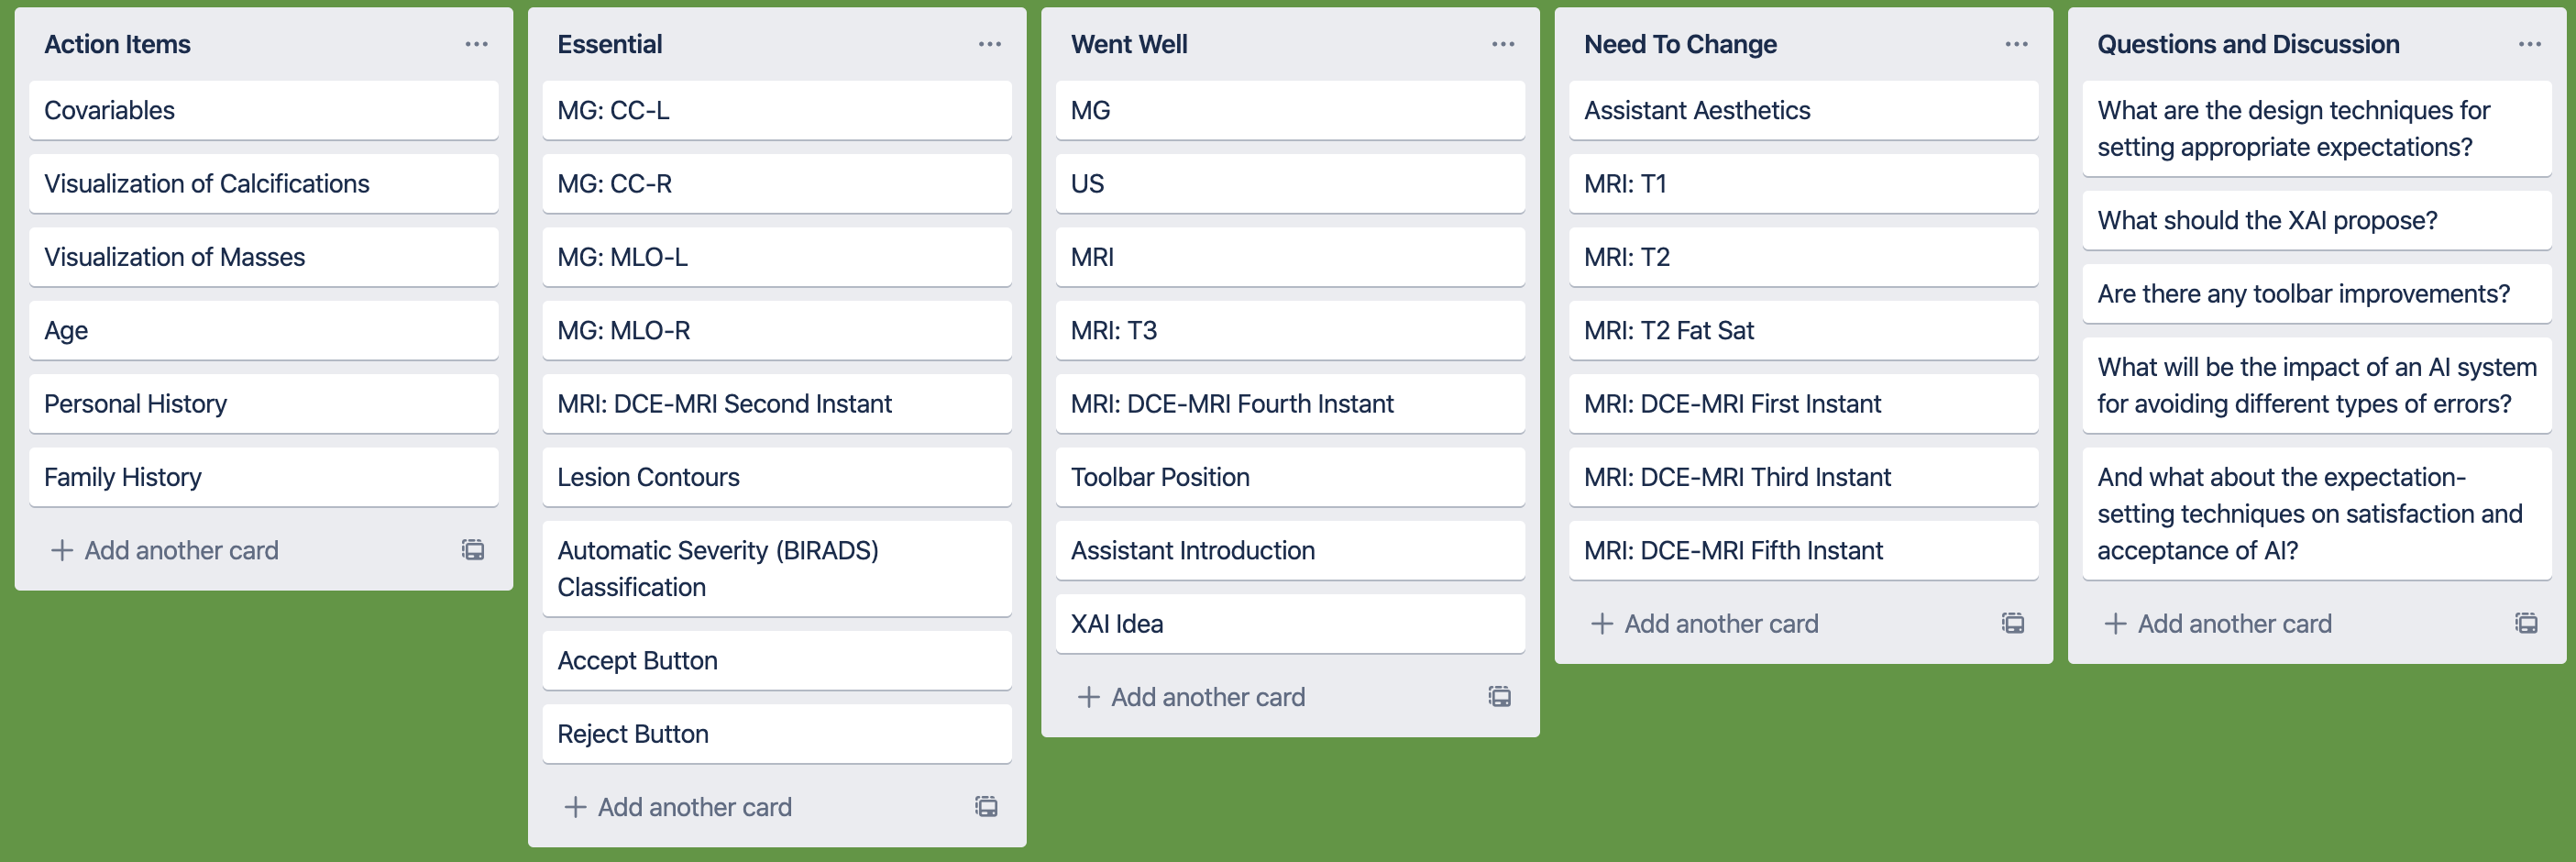
\includegraphics[width=\columnwidth]{images/fig039}
\caption{Resulting affinity diagrams passed to a digital software tool. The overall ideas and functionalities for categorization. Each idea and functionality has a category ({\it e.g.}, ``Action Items'', ``Essential'', ``Went Well'', ``Need To Change'' or ``Questions and Discussion''), so that it can manage the final requirements and development priorities of the {\it Assistant}.}
\label{fig:fig039}
\end{figure}
%%%%%%%%%%%%%%%%%%%%%%%%%%%%%%%%%%%%%%%%%%%%%%%%%%%

From workshops (Section~\ref{sec:chap005003003001}), participants ({\it i.e.}, researchers and some of the clinicians) of the focus group (Section~\ref{sec:chap005003003002}), were asked to review and re-position ideas and functionalities, within each category, in order to organize them.
Every time an idea or functionality was triggered, it was inserted into the ``Action Items'' category.
After that, participants discuss where it should be, answering the workshop needs for item categorization.
For instance, several clinicians listed\footnotemark[8] their preferred components as the position (32/45) and simplicity (28/45) of the {\it Toolbar} (Section~\ref{sec:chap005004002}):
``The {\it Toolbar} position should be on the top in contrary to what we usually see'' (C30).
From here, an item was created titled as ``Toolbar Position'' and since it was accepted by a major number of clinicians (and rejected or omitted by a minor number) the item was stuck onto the ``Went Well'' category.

%%%%%%%%%%%%%%%%%%%%%%%%%%%%%%%%%%%%%%%%%%%%%%%%%%%
\footnotetext[8]{The workshop answers and feedback were transcribed so that they can join with similar opinions in different items. A ``(32/45)'' means that 32 clinicians for a total of 45 clinicians appointed a similar sentence of the clinician number 30, {\it i.e.}, ``(C30)'' on that example.}
%%%%%%%%%%%%%%%%%%%%%%%%%%%%%%%%%%%%%%%%%%%%%%%%%%%

\vspace{0.05mm}

\noindent
Through the affinity diagrams, it was found that specific items, within each own categories, correspond to three needs of clinicians:

\vspace{0.10mm}

%%%%%%%%%%%%%%%%%%%%%%%%%%%%%%%%%%%%%%%%%%%%%%%%%%%
\begin{enumerate}[label=\alph*]
\item - new strategies among the medical imaging visualizations;
\item - to understand the intelligent agent ({\it Assistant}) result; and
\item - to control ({\it e.g.}, {\it accept} or {\it reject}) the final intelligent agent ({\it Assistant}) result.
\end{enumerate}
%%%%%%%%%%%%%%%%%%%%%%%%%%%%%%%%%%%%%%%%%%%%%%%%%%%

\vspace{0.10mm}

These threefold clinicians' needs were possible to achieve due to the correct application of affinity diagrams.
The technique was of chief importance to promote an understanding of this thesis background (Chapter~\ref{chap:chap002}).
Without such an approach, it would be impossible to follow the proper design of the developed intelligent agent.
Furthermore, the technique will follow all the steps and iterations that will be important for the future directions of this thesis (Section~\ref{sec:chap007004} of Chapter~\ref{chap:chap007}).

During the focus group, clinicians identified the need to map out all {\it workflow} processes and activities required to complete the diagnostic pipeline.
This highlighted the importance of introducing \ac{AI} systems taking into account these {\it workflow} characteristics to assist with their clinical tasks.
One clinician even stated that an intelligent agent would make their job more straightforward:
``If we have an intelligent assistant like this in our workflow, it will be more simple and easy to do our job'' (C45).
The identified needs included all the preconditions that facilitate prompt diagnosis.

Throughout this process, a set of design guidelines have been derived.
In order to investigate how the clinical {\it workflow} proceeds, affinity diagrams were used to connect ideas and features to a set of guidelines that will be described next.
For this purpose, three central design components were created that can be applied for medical imaging systems with \ac{AI} behind:
(i) highlighting the essential lesion regions;
(ii) explaining the \ac{AI} results for higher interpretability; and
(iii) providing control of the final result.
As follows, these three design components are translated into four design guidelines.

\noindent
From Figure~\ref{fig:fig039} and from the feedback obtained when building the affinity diagrams, the following design guidelines were considered:

\vspace{1.00mm}

%%%%%%%%%%%%%%%%%%%%%%%%%%%%%%%%%%%%%%%%%%%%%%%%%%
\begin{description}
\item[Relevance to Diagnostic] - the \ac{AI} system ({\it Assistant}) should provide additional relevant clinical information so that clinicians can explore more granular details of the diagnosis.
For instance, information that allows clinicians to understand the relevant lesions (Figure~\ref{fig:fig032}) and the respective severity levels regarding both the shape and size of the lesion.

\vspace{1.50mm}

\item[Clinician-Centered Activities] - since data must be shared between clinicians, the \ac{AI} system should be designed to mimic collaboration.
For instance, clinicians should be able to remotely visualize the same lesion annotation synchronously.
This means the \ac{AI} system should support and enhance activities that facilitate discussion, leading to more robust decision-making.

\vspace{1.50mm}

\item[Provide Explanations] - the system must provide answers regarding the final \ac{AI} result.
In this work, an ``Explain'' button (Figure~\ref{fig:fig040}) was created so that clinicians can open the heatmaps (Figure \ref{fig:fig032}) on the image.
The heatmaps will show the variability (color) of the important regions, which is information that will explain the final \ac{BI-RADS}.

\vspace{1.50mm}

\item[Feeling in Control] - the {\it Assistant} must provide control for the final decision. Clinicians must feel that, in case of a wrong \ac{AI} diagnostic, the final result must be changed ({\it reject}) by them so that we can guarantee the patient's safety and the right treatment of the lesion.
\end{description}
%%%%%%%%%%%%%%%%%%%%%%%%%%%%%%%%%%%%%%%%%%%%%%%%%%

\vspace{2.00mm}

Next (Section~\ref{sec:chap005003003004}), the document describes how the clustering of acquired data was essential.
The importance of clustering is based on the {\it affinity} of the collected ideas and functionalities.
The clustering process allowed us to identify common themes and patterns in the data, which were used to inform the design guidelines for the proposed medical assistant.
By clustering the ideas and functionalities, we could distill the large amount of data collected from the interviews and workshops into a smaller set of key design components that could be applied to medical imaging systems with \ac{DL} models behind.

\subsubsection{Essential Data}
\label{sec:chap005003003004}

Analyzing the essential data is vital for the developed \ac{UI}.
Indeed, the \ac{MRI} data is inherently chaotic since each exam contains tens of volumes.
The volumes can be part of several sequences\footnotemark[9] for the \ac{MRI} modality.
Thus, designing a comprehensive visualization for such chaotic data is necessary.

%%%%%%%%%%%%%%%%%%%%%%%%%%%%%%%%%%%%%%%%%%%%%%%%%%
\footnotetext[9]{As the most sensitive method for detection of breast cancer (\href{https://radiopaedia.org/articles/breast-mri?lang=us}{radiopaedia.org/articles/breast-mri}), the breast MRI aims to obtain a reliable evaluation of any lesion within the breast. However, the modality relies on several sequence options, such as: (1) T1 (longitudinal relaxation time), the time constant which determines the rate at which excited protons return to equilibrium; (2) T2 (transverse relaxation time), similar to T1, but with the second time constant; (3) T2 Fat-Sat, pulses are short-duration tuned to the resonance frequency of fat; (4) T2 Turbo Inversion Recovery Magnitude (TIRM); (5) Diffusion, method that produces invivo MRI of tissues sensitized with the local characteristics of molecular diffusion; (6) DCE Maximum Intensity Projection (MIP); (7) DCE WithOut (WO) contrast agent; and (8) DCE Positive Enhancement Integral (PEI). Although they are more, these were the MRI sequence options used by the nine institutions. Nevertheless, it is important to underline that the MRI volumes are always used as an adjunct to the standard diagnostic procedures of the breast, {\it i.e.}, clinical examination, MG and US.}
%%%%%%%%%%%%%%%%%%%%%%%%%%%%%%%%%%%%%%%%%%%%%%%%%%

\noindent
Specifically, for the medical imaging background (Chapter~\ref{chap:chap002}), the following \ac{MRI} characteristics were addressed:

\vspace{0.05mm}

%%%%%%%%%%%%%%%%%%%%%%%%%%%%%%%%%%%%%%%%%%%%%%%%%%
\begin{multicols}{4}
\begin{enumerate}
\item T1;
\item T2;
\item T2 Fat-Sat;
\item T2 TIRM;
\item Diffusion;
\item DCE MIP;
\item DCE WO;
\item DCE PEI;
\end{enumerate}
\end{multicols}
%%%%%%%%%%%%%%%%%%%%%%%%%%%%%%%%%%%%%%%%%%%%%%%%%%

\vspace{0.05mm}

The process of clustering notes based on their {\it affinity} to a shared topic helps to create data groups, which are recursively labeled and clustered until the highest level has only a few groups~\cite{harrington2016affinity}.
This leads to the identification of common issues and potential solutions, helping to frame user needs and design problems.
The approach supported the final design and development decisions for the intelligent agent, resulting in an optimized solution that meets user needs.

During the focus groups (Section~\ref{sec:chap005003003002}), participants identified several user needs and requirements that were crucial ({\it i.e.}, ``Essential'' column of Figure~\ref{fig:fig039}) in defining the most critical modalities and procedures for the medical imaging workflow (Figure~\ref{fig:fig018}).
With several \ac{MRI} sequences available, clinicians face the ``chaotic data problem'' of visualizing all the volumes.
Therefore, it is essential to identify the \ac{MRI} volumes that best match the clinicians' needs.
This process is supported by affinity diagrams and the resulting user needs and requirements, which help define essential modalities and procedures for the workflow.

We also observed that clinicians from different hospitals had different preferences for \ac{MRI} sequences.
However, since the medical imaging data used was from the \acs{HFF} clinical institution, their main sequence (\acs{DCE-MRI} in a second instant) was chosen as the standard.
Through data clustering, the need for each modality (\acs{MG}, \acs{US} and \acs{DCE-MRI} at the second time instant) and its meaning to the clinical workflow (Figure~\ref{fig:fig018}) were identified.
The workshops (Section~\ref{sec:chap005003003001}) and focus groups (Section~\ref{sec:chap005003003002}) helped to gather essential data on how these modalities can provide complementary information for a reliable diagnosis, tailored to each institution's needs.

\subsubsection{Prototype Requirements}
\label{sec:chap005003003005}

From our human-centered approach, we conclude that the \ac{AI}-assisted prototype should consist of two parts:
(1) the diagnosis via multi-modal medical imaging, in which the proposed prototype has several functionalities to support clinicians with tools prioritized during our design interventions; and
(2) the automatic severity classification of lesions, in which a DenseNet is integrated as an anthropomorphic intelligent agent providing the \ac{BI-RADS} scores and explanations.
Due to workshops and focus groups, it is possible to explore in a higher manner the good insights of clinicians.
At this study stage, several clinicians provided necessary modifications and feedback for the future system.
For instance, bringing the intelligent agent from the top and middle to the button right of the screen inside the {\it 5.1. Viewports} (Figure~\ref{fig:fig040}).
Again, the comment was provided during the design activities at this phase.

We expect that some suggestions will improve clinicians' decision-making, while reducing the total time to diagnose a patient (Section~\ref{sec:app003004005} of Appendix~\ref{chap:app003}) over interaction, as well as the medical error.
From the proposed design activities, we could understand that the {\it 6. Assistant} avatar must be placed inside the {\it 5.1. Viewports} (Figure \ref{fig:fig040}), making the intelligent agent easily accessible without compromising visibility.
The explanation was simple, clinicians are used to work inside the {\it 5.1. Viewports} (Figure \ref{fig:fig040}).
Meaning that it is less distance, time, and effort to interact with the {\it 6. Assistant} avatar.
Furthermore, the visibility was not compromised because of two reasons:
(a) first, most of the cases (typically the majority of \ac{MG}, and \ac{MRI} modalities) has no relevant image information on the button right of the screen inside the {\it 5.1. Viewports}; and
(b) we developed a hidden button, so that if a clinician really needs to look at that area, the {6. \it Assistant} avatar will disappear, showing the full image with nothing overlaid.
By incorporating these design choices (Section~\ref{sec:app003003001}), the intelligent agent is not only more accessible, but also better integrated into the clinicians' existing workflow.
This sets the stage for the investigation of how \ac{AI}-assisted methods can be integrated into the design of intelligent agents, which we explore in the following section (Section~\ref{sec:chap005003003}).
Specifically, we focus on how the design of {\it BreastScreening-AI} can help mitigate breast cancer diagnosis while meeting overall design goals in healthcare.

\subsection{Design Goals}
\label{sec:chap005003004}

In this section, it is investigated how \ac{AI}-assisted methods could be integrated into the design of an intelligent agent for the medical imaging diagnostic on breast cancer.
The purpose is to help mitigate breast cancer diagnosis, while meeting overall design goals.
This solution provides an absolute scale for clinicians' performance and leads to the instrumentation of the hereby design goals and constrains.
With the introduction of intelligent agents, the designed {\it BreastScreening-AI} framework~\cite{CALISTO2021102607} dictated a departure from the later {\it BreastScreening} annotating tool~\cite{10.1145/3399715.3399744} wrapping approach of \ac{AI} techniques, toward a new communication that only exposes the required patient information, as well as lesion classification and segmentation functionalities (Appendix~\ref{chap:app008}).
The {\it BreastScreening-AI} framework is designed to reduce the burden of usage and expand clinicians' performance by simplifying the complexities that are frequently encountered when clinicians are diagnosing a patient.
Here, the main goal is to expose the \ac{AI} algorithm results in a readily available format~\cite{CALISTO2022102285}.
The design goals of {\it BreastScreening-AI} have been for a robust, reliable, and elegant \ac{UI} to promote the integration of intelligent agents in the \ac{RRR} workflow.

The main design goals are closely related to the research insights and challenges of the previous section (Section~\ref{sec:chap005003002}), namely:
(1) collection of a \ac{GT} annotations, {\it i.e.}, masses in all imaging modalities and microcalcification lesions in \ac{MG} (for both \ac{CC} and \ac{MLO} views);
(2) classification of the lesion severity using the \ac{BI-RADS}~\cite{aghaei2018association};
(3) categorization of the breast tissues (dense vs non-dense);
(4) clinical co-variables, such as personal and family records; and
(5) visualizations for clinical summary which are crucial for a proper diagnosis and to perform patient follow-up.

\noindent
These five insights were fused into three corresponding design goals, as follows:

\vspace{1.00mm}

%%%%%%%%%%%%%%%%%%%%%%%%%%%%%%%%%%%%%%%%%%%%%%%%%%
\begin{description}
\item[\ac{MID}] focusing on how to provide the best visualization strategy, given the heterogeneous information coming from the multi-modal nature of the information;

\vspace{0.50mm}

\item[\ac{CRD}] focusing on improving the clinician's ability to {\it accept} or {\it reject} the \ac{AI}-assisted results;

\vspace{0.50mm}

\item[\ac{EXD}] focusing on increasing physician's understanding of how the \ac{AI} techniques operate. By increasing understanding of how \ac{AI} works, physicians can update their expectations of how well and in which situations the system is likely to work;
\end{description}
%%%%%%%%%%%%%%%%%%%%%%%%%%%%%%%%%%%%%%%%%%%%%%%%%%

\vspace{1.50mm}

Until now, this is the first attempt to holistically integrate these design goals in the context of medical imaging diagnosis supported by \ac{AI}-assisted methods.
Through user studies, it was identified the above three ({\it i.e.}, \ac{MID}, \ac{CRD} and \ac{EXD}) design goals.
Next, the document will describe the {\it BreastScreening-AI} framework~\cite{CALISTO2021102607} taking into account these design goals.

\section{BreastScreening-AI}
\label{sec:chap005004}

To validate the proposed design goals, a prototype called {\it BreastScreening-AI} framework was developed~\cite{CALISTO2021102607}.
As a proof-of-concept fully functional prototype, this tool aims to be evaluated in a realistic clinical scenario.
In the following sections, the document will describe the main functionalities for prototyping the {\it BreastScreening-AI} framework.
Next, the document describes the prototype details and system implementation.

\subsection{Implementation}
\label{sec:chap005004001}

Similar to an earlier version, the {\it BreastScreening-AI} framework was implemented using \href{https://cornerstonejs.org/}{CornerstoneJS} with a \href{https://nodejs.org/}{NodeJS} server.
Once the set of medical images is loaded in the visualization viewport (Figure \ref{fig:fig040}) the user can interact with the data by manipulating the visualization through the mouse and keyboard.
For instance, rolling the mouse wheel to navigate across the volume slices (\acs{MRI}) or even moving the mouse to drag-and-drop the several modalities to the viewport.
The goal of the proposed multi-modal strategy is then to provide the visualization and manipulation of several modalities, comparing lesion patterns among medical images.

Due to the integration of intelligent agents, the new developments of the {\it BreastScreening-AI} prototype were giving this thesis the opportunity to test properly what are the implications of \ac{AI} techniques on the \ac{RRR} workflow.
Such implications are achieved through the implementation and integration of a classifier model (DenseNet) into the designed \ac{UI}~\cite{maicas2018training}.
By showing the work design decisions, the following sections will cover these prototyping directions.

%%%%%%%%%%%%%%%%%%%%%%%%%%%%%%%%%%%%%%%%%%%%%%%%%%%
\begin{figure}[htbp]
\centering
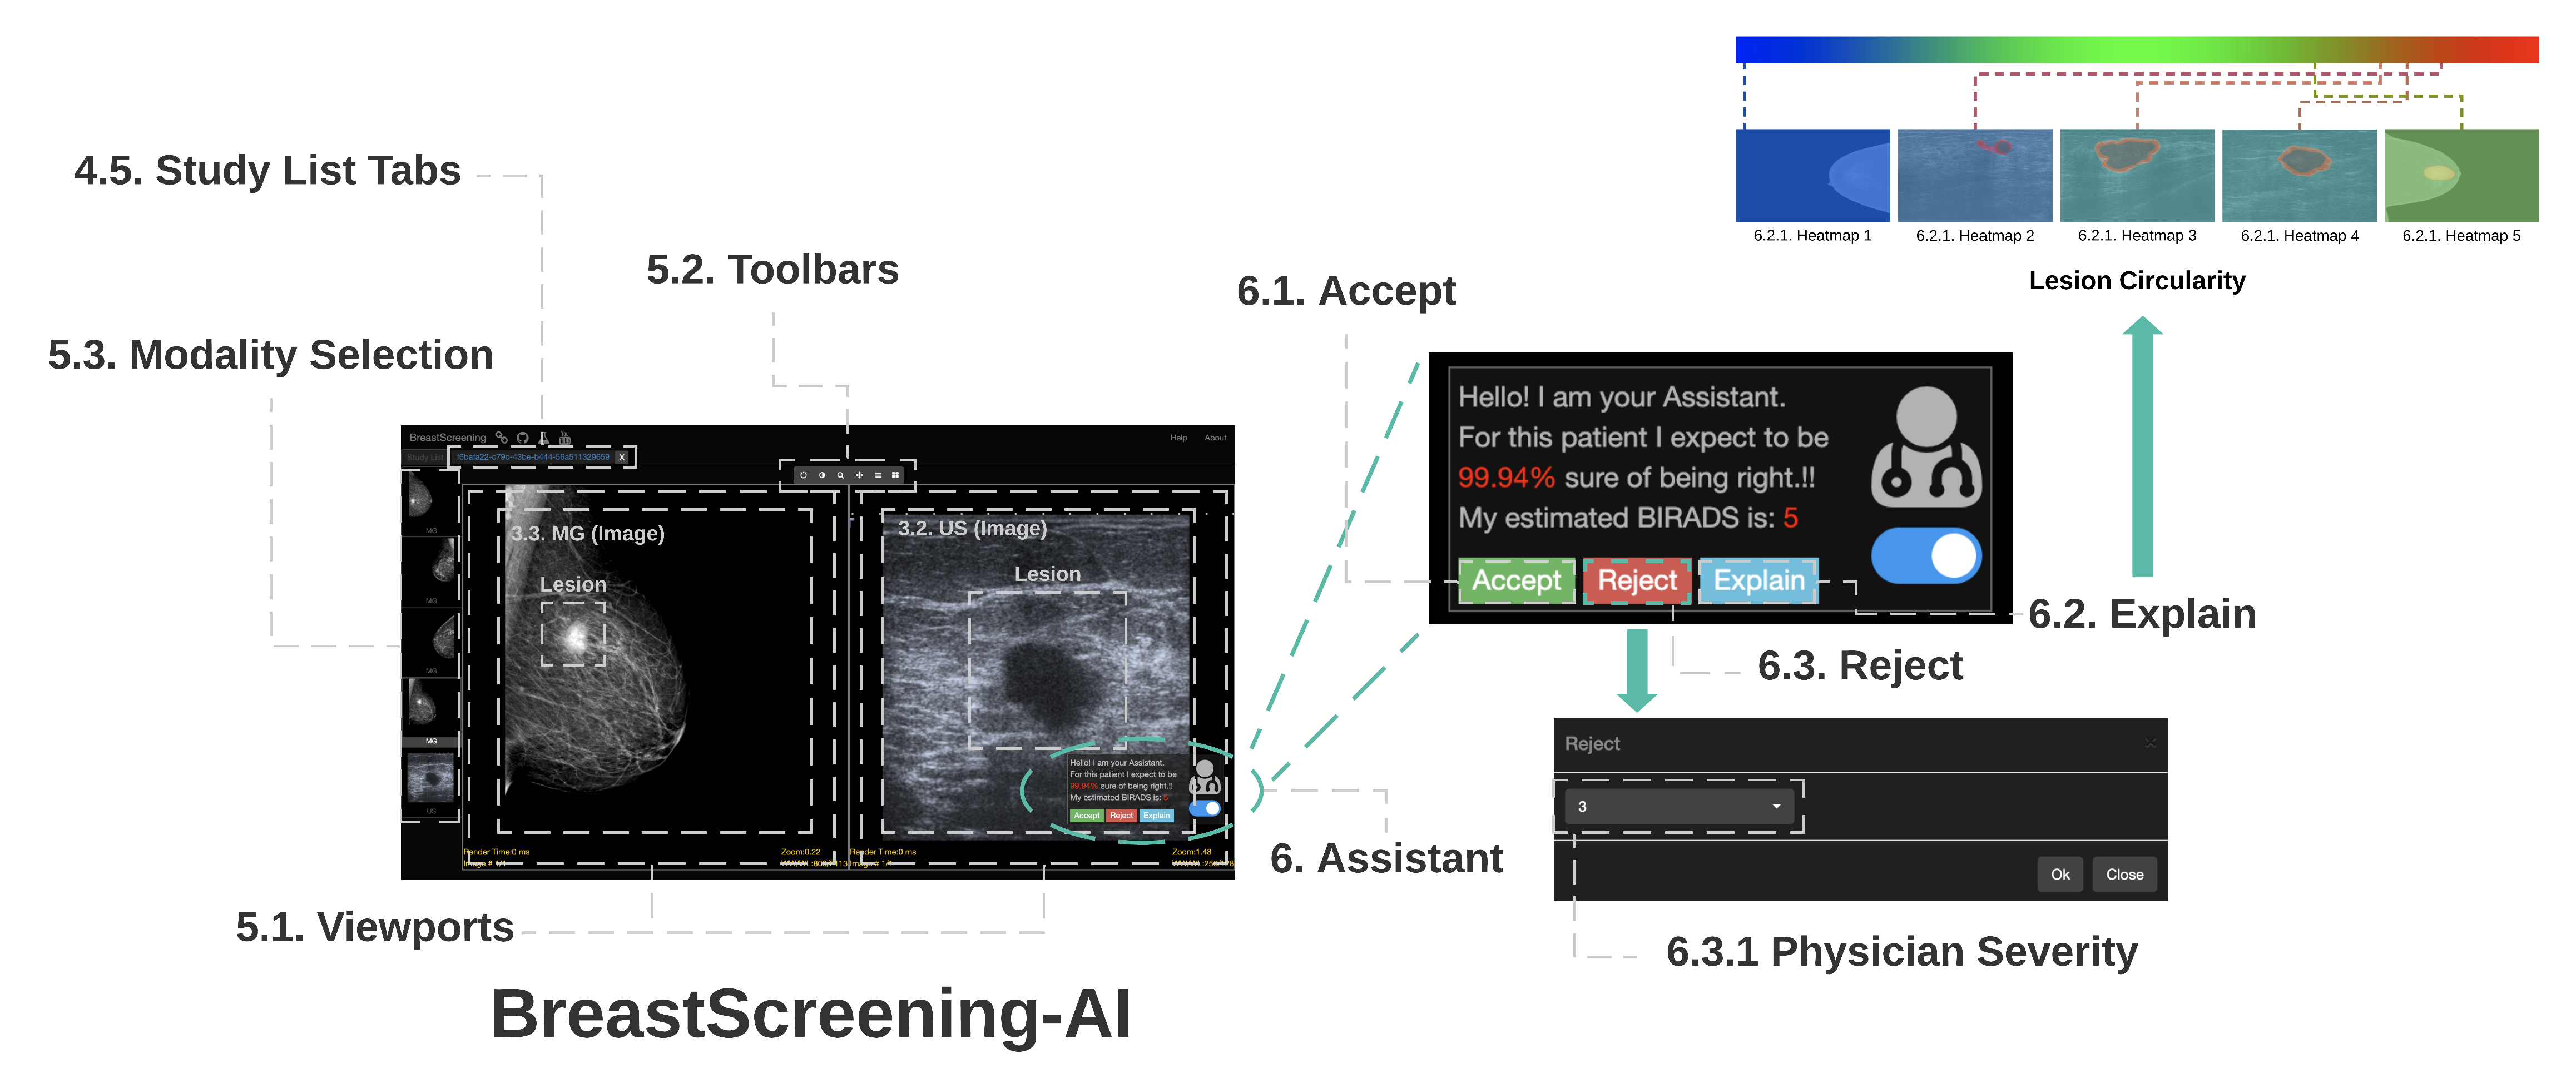
\includegraphics[width=\textwidth]{images/fig040}
\caption{The proposed {\it BreastScreening-AI} provides several functionalities. Specifically, it is possible to validate the DenseNet output classification along with radiologists. The system is framed in the following subcategories: 4.5. Study List Tabs; 5.1. Viewports; 5.2. Toolbars; 5.3. Modality Selection; 6. Assistant; 6.1. Accept; 6.2. Explain; 6.3. Reject; and 6.3.1. Physician Severity. On 6.2. Explain, the assistant will pop-up several heatmaps. The proposed model has two main stages: (i)  first it computes the BI-RADS, based on the output classification of the DenseNet; and (ii) it computes the size and circularity of the lesion based on the heatmaps.}
\label{fig:fig040}
\end{figure}
%%%%%%%%%%%%%%%%%%%%%%%%%%%%%%%%%%%%%%%%%%%%%%%%%%%

\subsection{User Interface}
\label{sec:chap005004002}

In this section, we describe the design and implementation of the \ac{UI} for the {\it BreastScreening-AI} prototype based on identified user needs (Section~\ref{sec:chap005003003}).
The \ac{UI} includes a set of refinement mechanisms to guide clinicians during the diagnostic process (Figure~\ref{fig:fig040}), comprising two main components:
(1) the list of patients; and
(2) medical imaging views.
The {\it 4. List of Patients Views} include a {\it 4.1. List of Patients} with the most important and required information for clinicians.
From here, users can search all patients using criteria such as {\bf Patient ID}, {\bf Study Date}, available {\bf Modality} sets, {\bf Study Description}, and number of {\bf Images}.
The {\it 4.5. Study List Tabs} allow clinicians to switch between diagnosed patients and medical imaging diagnosis views.
The \ac{UI} is also informing clinicians about how to classify and use the system, {\it 5.2. Toolbars} to match the user's requirements, and {\it 5.1.~Viewports} to process the image by using {\it 5.2. Toolbars} provided functionalities.
In the end, the \ac{BI-RADS} functionality ({\it 6.3.1.~Physician Severity}) allows clinicians to classify the severity of the breast lesion for each patient.

Overall, this section describes the design and implementation of the \ac{UI} for prototyping the first iterations of the {\it BreastScreening-AI} framework.
Specifically, it includes refinement mechanisms to guide clinicians during the diagnostic process.
The following sections will map the two main \ac{UI} functionalities, {\it i.e.}, assistant (Section~\ref{sec:chap005004002001}) and explainability (Section~\ref{sec:chap005004002002}), between the design goals (Section~\ref{sec:chap005003002}) under this thesis.

\subsubsection{Assistant}
\label{sec:chap005004002001}

The {\it 6.1.~Accept} or {\it 6.3.~Reject} (Figure~\ref{fig:fig040}) allows the clinician to accept or reject the automatic classification of the {\it 6.~Assistant}.
The {\it 6.~Assistant} is based on the outcomes of a DenseNet~\cite{Huang_2017_CVPR}.
However, integrating a \ac{DNN} needs special attention (Appendix~\ref{chap:app004}).
Typically, the training of a \ac{DNN} is expensive regarding the time spent (Section~\ref{sec:app004001}), since its classification performance will improve as the training dataset becomes larger.
Thus, training the model from scratch is not the best option.
For this reason, we pre-train ({\it i.e.}, off-line training before the \ac{UI} integration) the \ac{DNN} on the ImageNet dataset~\cite{10.1145/3351095.3375709} and fine-tuned using our multi-modal breast dataset (Section~\ref{sec:app004005}).
Specifically, we fine-tune the \ac{DNN} using supervised learning.
Only afterwards, the pre-trained DenseNet is incorporated into the \ac{UI}.

The implemented DenseNet takes medical images as an input and outputs the severity probability.
The input consists of images ({\it i.e.} \ac{MG}, \ac{US} and \ac{MRI} slices) with the corresponding label ({\it i.e.}, the \ac{BI-RADS}) that is previously classified by an expert.
The output consists of having five nodes in the last layer of the \ac{DNN}.
Each node is assigned to a given class that corresponds to each \ac{BI-RADS} score.
After this stage, we have conditions for the integration, since now the DenseNet is tuned to perform the classification in unseen test images.
The classification is fast, being tailored for an online diagnosis.

When several modalities (\ac{MID} and \ac{CRD}) are correctly used (regarding the {\it 5.3.~Modality~Selection} on a multimodality view), the clinician can find more accurately the right severity classification, as concluded in Section~\ref{sec:app003003002} of Appendix~\ref{chap:app003}.
For the {\it 6.3.~Reject} option, the physician will have the opportunity to insert (\ac{CRD}) the proposed \ac{BI-RADS} on a drag-and-drop menu ({\it 6.3.1.~Physician Severity}) of severity options.
Both \ac{MID} and \ac{CRD} goals are supporting our {\bf RQ5.1} question (Section~\ref{sec:chap005001002}).

\subsubsection{Explainability}
\label{sec:chap005004002002}

Finally, the clinician may press for the {\it 6.2.~Explain} functionality  by looking at the generated heatmaps (Figure~\ref{fig:fig032}).
The generation of the above colour maps come from the following information: (i) the area ({\it Lesion Size}) of the lesion that comes from the delineation process, (ii) the circularity/sharpness ({\it Lesion Shape}) that can be computed from the annotation in (i), and (iii) the \ac{BI-RADS} score automatically provided by the DenseNet ({\it i.e.}, classifier intelligent agent).
The \ac{EXD} design goal is performed as above described helping to answer to research questions {\bf RQ5.2} and {\bf RQ5.3} (Section~\ref{sec:chap005001002}).

Covered by the \ac{EXD} design goal, the thesis can provide a key component to disambiguate the \ac{AI} result with the application of an explanation technique (Section~\ref{sec:chap003007}).
For a better prediction, the result of this explanation process is a heatmap visualizing the importance of each pixel.
With heatmaps, clinicians can capture and understand the logic arguments of the DenseNet (Section~\ref{sec:chap005006002}) by giving images and pixels a colour meaning of the lesion severity.
Thus, the \ac{EXD} design goal is bringing the opportunity to disambiguate this \ac{DL} method for more transparent and explainable (\ac{XAI}) process.
Next, the section will describe the applied study methods to prove these claims.


%%%%%%%%%%%%%%%%%%%%%%%%%%%%%%%%%%%%%%%%%%%%%%%%%%%
\begin{figure}[htbp]
\centering
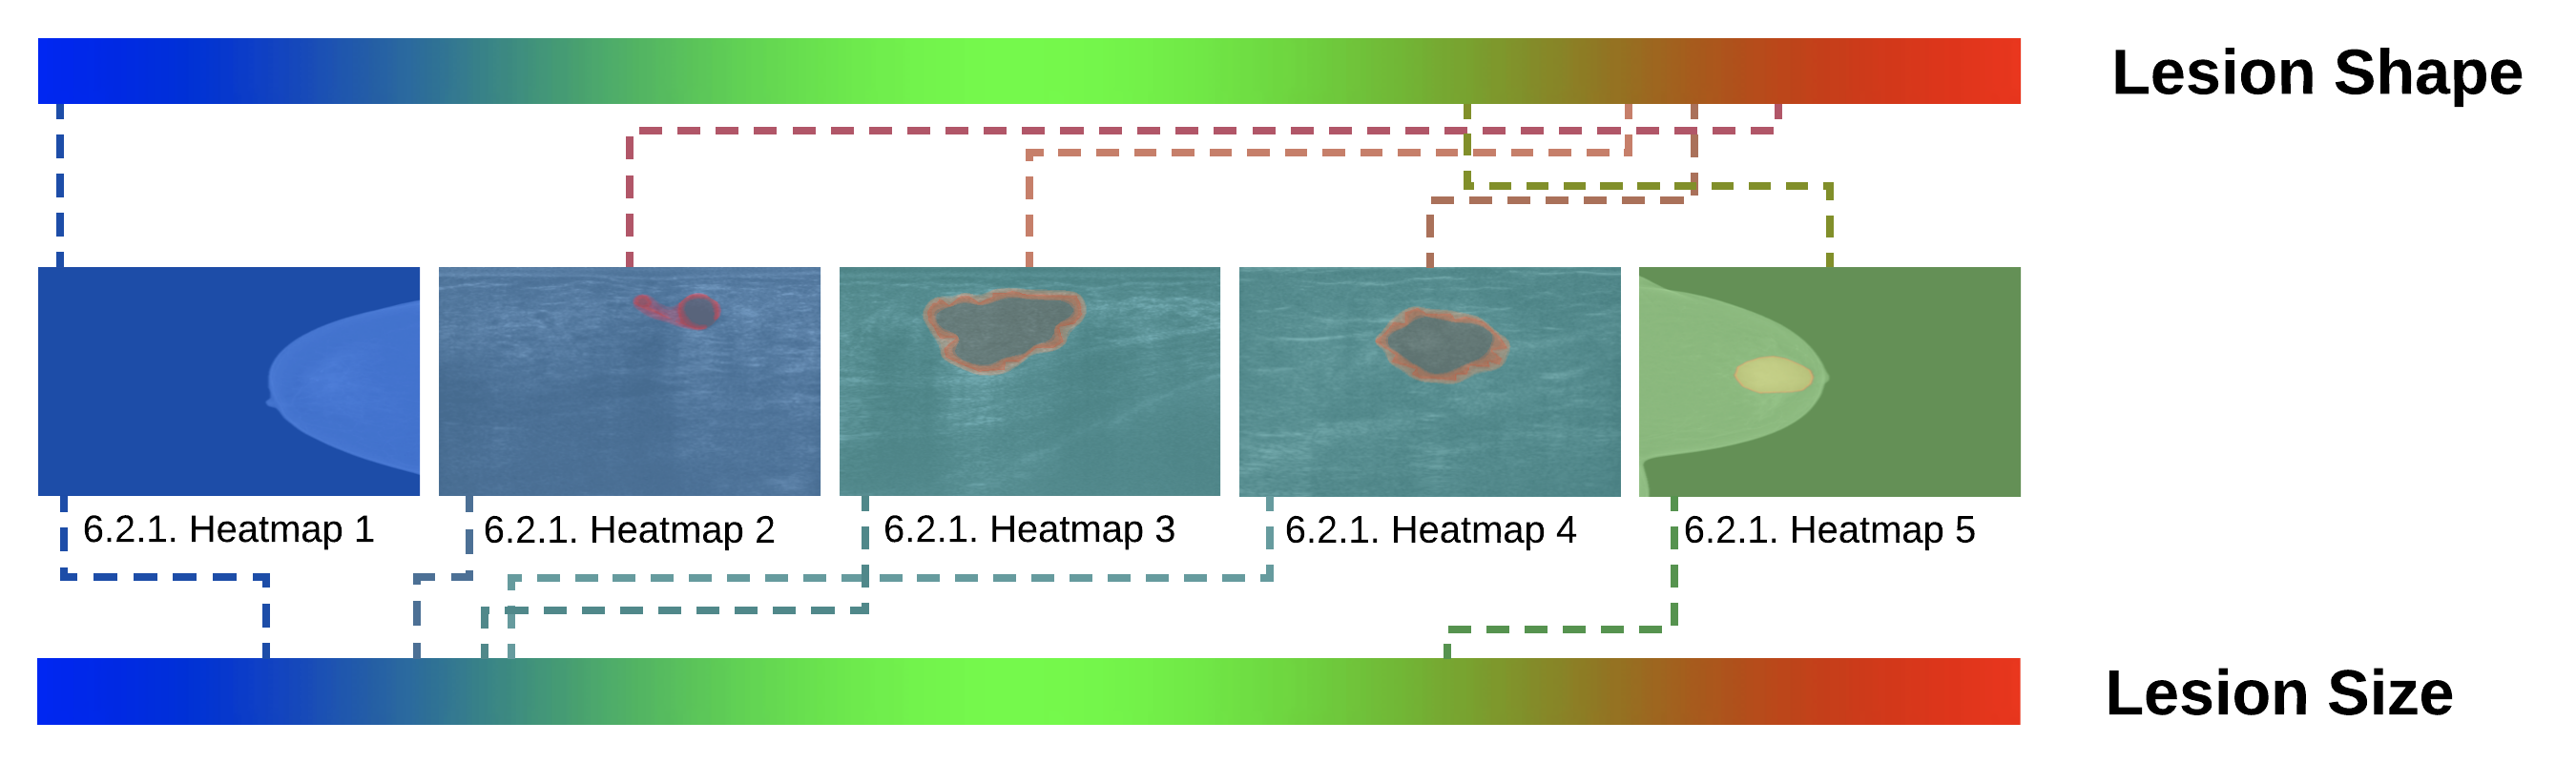
\includegraphics[width=\columnwidth]{images/fig032}
\caption{On {\it 6.2.~Explain}, the assistant will pop-up several {\it heatmaps}. The {\it heatmaps} represent two different scales: (a) {\it Shape}; and (b) {\it Size} of the lesion. First, the model computes the BI-RADS using the DenseNet classification. Second, the model computes the lesion circularity (top scale) and size (bottom scale) and associate it to the colors regarding both circularity/size and BI-RADS.}
\label{fig:fig032}
\end{figure}
%%%%%%%%%%%%%%%%%%%%%%%%%%%%%%%%%%%%%%%%%%%%%%%%%%%

\section{Methods}
\label{sec:chap005005}

For this study, an evaluation of {\it BreastScreening-AI} simulating real-world conditions with 45 clinicians, within-subject, in nine different clinical institutions was conducted.
The study goal was to quantitatively and qualitatively assess the proposed design principles that the {\it BreastScreening-AI} embodies, and to understand how these principles would work in practice.
The experimental setup aimed at testing two conditions: {\bf Clinician-Only} ({\it Current}) -- simulating clinicians' {\it current} setup, equal to what they have in their clinical institutions, {\it i.e.}, a multimodality strategy without any \ac{AI}-assisted technique; {\bf Clinician-AI} ({\it Assistant}) -- multimodality strategy taking advantage of the \ac{AI}-assisted ({\it e.g.}, DenseNet~\cite{9098470}), supporting clinician's second opinion and autonomous patient diagnostic.

\vspace{2.00mm}

\noindent
For each condition, three classes of patients were defined:

%%%%%%%%%%%%%%%%%%%%%%%%%%%%%%%%%%%%%%%%%%%%%%%%%%%
\begin{itemize}
\item {\bf Class 1}: patients such that \ac{BI-RADS} $\leq$ 1 (low severity);
\item {\bf Class 2}: patients such that 1 $<$ \ac{BI-RADS} $\leq$ 3 (medium severity);
\item {\bf Class 3}: patients such that \ac{BI-RADS} $>$ 3 (high severity);
\end{itemize}
%%%%%%%%%%%%%%%%%%%%%%%%%%%%%%%%%%%%%%%%%%%%%%%%%%%

Having data available is challenging and requires multiple steps (Section~\ref{sec:app004002}), including anonymization of data.
The ideal approach is a collaboration between clinicians and \ac{AI} researchers, either in-house or through collaborative research agreements.
Therefore, a protocol was celebrated with \acs{HFF} so that the interchange of patients could be possible.
The purpose of this protocol is to establish bases of collaboration in all scientific and technological areas, as well as education and training in which \ac{IST} and \acs{HFF} carry out their activities.
From this protocol, the exams were annotated by eight radiologists and classified with a \ac{BI-RADS} severity from an expert doctor.
The expert doctor is the head of the radiologist services of the \acs{HFF} clinical institution.

\subsection{Participants}
\label{sec:chap005005001}

In this study, participants were asked to practice with three predefined sets of patients randomly selected from the three above classes.
To accomplish this, each patient was randomly selected ({\it i.e.}, {\bf P1}, {\bf P2} and {\bf P3}) from each class ({\it i.e.}, {\bf Class 1}, {\bf Class 2} and {\bf Class 3}), respectively.
Then, participants were asked to diagnose each patient.
A natural expectation is that the intelligent agent would minimize the time required and accuracy ({\it e.g.}, improving \ac{FP} or \ac{FN} values).
The study involved 45 clinicians, recruited on a volunteer basis from a broad range of clinical scenarios, including nine different health institutions (two public hospitals, two cancer institutes, one private hospital, and two private clinics).

\vspace{4.00mm}

\noindent
In the following list, the number of clinicians and respective clinical institutions is provided:

\vspace{2.00mm}

\begin{multicols}{2}
\begin{itemize}
\item 12 clinicians of \acs{HFF};  % HFF
\item 10 clinicians of \acs{IPOL}; %IPOL
\item 2 clinicians of \acs{HSM};   %HSM
\item 9 clinicians of \acs{IPOC};  %IPOC
\item 1 clinician of \acs{MMC};    %MMC
\item 1 clinician of \acs{SAMS};   %SAMS
\item 8 clinicians of \acs{HB};    %HB
\item 1 clinician of \acs{HSA};    %HSA
\item 1 clinician of \acs{JCCC}.   %JCCC
\end{itemize}
\end{multicols}

\vspace{2.00mm}

Before the experiment, clinicians first filled out a pre-study questionnaire eliciting demographic information (Appendix~\ref{chap:app006}), including age group, gender, and medical professional experience, among others.
From the demographic questionnaires:
24.4\% of the clinicians have between 31 and 40 years of practical experience (seniors);
31.1\% have between 11 and 30 years of experience (middles);
17.8\% have between 6 and 10 years of experience (juniors); and
26.7\% have limited experience (interns).
Interviews were conducted in a semi-structured fashion, taking about 30 minutes.
Overall, 57 days were spent on the clinical institutions for the observation process and six months for the classification.

\subsection{Apparatus}
\label{sec:app002005002}

To track user interactions across the evaluated system, we used the \hyperlink{https://www.hotjar.com/}{Hotjar} tool.
This tool is an analytic package allowing this study to follow users remotely.
It also provides two critical pieces of functionality, among others, that can aid in remote user testing.
First, the frequency areas allow us to see where users are clicking, tapping and scrolling on the system.
Second, it records a video playback of the entire user session.
To record the task activities and the interview, the \hyperlink{https://support.apple.com/downloads/quicktime}{QuickTime} application was used for user's screen recording.
It was also useful for identifying any issues or errors that occurred during the user testing sessions.

Finally, to understand radiologists' reading behaviour an eye-tracking device was used while they were interacting with the intelligent agent.
The selected device was the \hyperlink{https://gaming.tobii.com/product/tobii-eye-tracker-4c/}{Tobii Eye Tracker 4C}, since Tobii is the largest commercial eye tracking manufacturer, and is one of the most common trackers among usability practitioners~\cite{CALISTO2021102607}.
Also, the \hyperlink{https://www.tobiipro.com/product-listing/tobii-pro-sdk/}{Tobii Pro SDK} was used, providing the thesis results with gaze information of the eye tracking device.

\subsection{Procedure}
\label{sec:chap005005003}

After providing informed consent for participation in the study, clinicians reported information about their demographics (age, gender, etc) and professional background (professional or academic training, number of years of clinical experience).
Next, clinicians familiarized themselves for about 30 seconds with \ac{UI} and with the basic interface components common to both Clinician-Only and Clinician-AI conditions (Section~\ref{sec:chap005005}).
However, the two conditions are different.

The first condition (Clinician-Only) relies on classifying patients without \ac{AI} assistance.
The goal was to understand what is the actual clinicians' performance.
Thus, a simulation of the current clinicians' available tools on the \ac{RRR} was held, while interacting with the first developed tool.

For the second condition (Clinician-AI), the procedure required to reject (or accept) the proposed \ac{BI-RADS} (Section~\ref{sec:app003003} of Appendix~\ref{chap:app003}) provided by the intelligent agent.
At this stage, participants will interact with the new framework ({\it i.e.}, the {\it BreastScreening-AI} prototype) using the multi-modal dataset acquired and curated under this thesis.
The test set is comprising a number of 289 patients (Section~\ref{sec:app003003004} of Appendix~\ref{chap:app003}).
In the dataset, there are cases where the patient does not have all the image modalities (recall Figure~\ref{fig:fig018} where the acquisition may finish before all the modalities are available).
Thus, the following requirements were defined to conduct the study work analysis.

\vspace{2.00mm}

\noindent
The requirements are as follows:

\vspace{0.05mm}

%%%%%%%%%%%%%%%%%%%%%%%%%%%%%%%%%%%%%%%%%%%%%%%%%%%
\begin{enumerate}
\item All patients must have each of the three available modalities;
\item All patients were annotated and classified by the radiology team of \acs{HFF};
\item The patients were grouped in low, medium, and high severity according to the \ac{BI-RADS};
\end{enumerate}
%%%%%%%%%%%%%%%%%%%%%%%%%%%%%%%%%%%%%%%%%%%%%%%%%%%

\vspace{0.05mm}

The above procedure allowed this work to obtain a set of 415 cases.
Notice that the dataset is partitioned according to the three classes mentioned above.
Similar for both conditions (Clinician-Only and Clinician-AI), the first task was to fill out pre-test forms, as already mentioned.
The second task was the user characterization form, providing participant demographic data.
Next, each participant accessed the system via a web browser.
Each of the 45 clinicians were assigned three patients ({\it e.g.}, {\bf P1}, {\bf P2} or {\bf P3}), for diagnosis.
Thus, for each clinician, it was assigned one patient with low severity, one with medium severity, and another one with high severity.

When analyzing the patients, for the second condition (Clinician-AI), the main task was to {\it accept} or {\it reject} the proposed \ac{BI-RADS} value provided by an intelligent agent.
This may increase the diagnostic time slightly.
In case of {\it rejecting} the proposed value, participants were asked to provide a new \ac{BI-RADS} value on the \ac{UI}.
An {\it explain} functionality was provided to be used informing participants concerning where and how much sever the lesions are (Figure~\ref{fig:fig032}).
However, for the first condition (Clinician-Only), the \ac{BI-RADS} classification was provided by clinicians in the end of patient analysis alongside filling a form (Appendix~\ref{chap:app006}).
These setups will be used to support the work results (Section~\ref{sec:chap005006}).

Before the main test, every interaction was shown by the facilitator, and upcoming questions were clarified (Appendix~\ref{chap:app007}).
In the end, for each participant it was applied both \ac{SUS}~\cite{Tyllinen:2016:WNN:2858036.2858570} and \ac{NASA-TLX}~\cite{10.1145/3399715.3399744} on two different questionnaires for usability\footnotemark[10] and workload\footnotemark[11] measurements.
Moreover, trust\footnotemark[12] is measured through three questions adapted from the Model of Trust~\cite{CALISTO2021102607} that is mentioned in this work as \ac{DOTS}.
Finally, a {\it post-task} questionnaire~\cite{10.1145/3132272.3134111} was carried out.

%%%%%%%%%%%%%%%%%%%%%%%%%%%%%%%%%%%%%%%%%%%%%%%%%%%
\footnotetext[10]{For SUS scores, we used a 5 item scale. The scores range from 1 - ``{\bf Strong Disagree}'' to 5 - ``{\bf Strong Agree}'' as a simple scale to measure usability. The mean across all individual questionnaires was computed over studies. We provide an available {\it dataset} (\href{https://mimbcd-ui.github.io/dataset-uta7-sus/}{mimbcd-ui.github.io/dataset-uta7-sus}) from our SUS data.}
%%%%%%%%%%%%%%%%%%%%%%%%%%%%%%%%%%%%%%%%%%%%%%%%%%%

%%%%%%%%%%%%%%%%%%%%%%%%%%%%%%%%%%%%%%%%%%%%%%%%%%%
\footnotetext[11]{For NASA-TLX scores, we used a 20 item scale. The scores range from 1 - ``{\bf Very Low}'' to 20 - ``{\bf Very High}'' with more item options to measure workload. Again, we provide an available {\it dataset} (\href{https://mimbcd-ui.github.io/dataset-uta7-nasa-tlx/}{mimbcd-ui.github.io/dataset-uta7-nasa-tlx}) from our NASA-TLX data.}
%%%%%%%%%%%%%%%%%%%%%%%%%%%%%%%%%%%%%%%%%%%%%%%%%%%

%%%%%%%%%%%%%%%%%%%%%%%%%%%%%%%%%%%%%%%%%%%%%%%%%%%
\footnotetext[12]{For DOTS scores, we used a 20 item scale comprised by three questions: \ac{DOTS}: (1) {\bf Understanding}: ``{\it I understand what the system is thinking}''; (2) {\bf Capability}: ``{\it The system seems capable}''; and (3) {\bf Benevolence}: ``{\it The system seems benevolent}''. The three questions were answered on a 20-point scale from ``{\bf 0\% - Totally Disagree}'' to ``{\bf 100\% - Totally Agree}'' with 5\% increments.}
%%%%%%%%%%%%%%%%%%%%%%%%%%%%%%%%%%%%%%%%%%%%%%%%%%%

\subsection{Analysis}
\label{sec:chap005005004}

In this study, we aim to understand user behavior during decision-making by taking into account differences between medical expert levels ({\it i.e.}, {\it Intern}, {\it Junior}, {\it Middle}, and {\it Senior}), user characteristics, and medical imaging interpretation.
The study included both quantitative (Section~\ref{sec:chap005005004001}) and qualitative (Section~\ref{sec:chap005005004002}) analyses.
The quantitative analysis focused on not only measuring usability, workload, and trust but also evaluating the radiologists' performance ({\it e.g.}, number of \acp{FP} and \acp{FN}) during diagnosis of three groups of patients ({\it i.e.}, low, medium, and high severity) for each doctor.
In addition, the qualitative analysis aimed to provide a more in-depth understanding of the radiologists' experience with the {\it BreastScreening-AI} prototype, including the feedback provided by clinicians on ease of use, usefulness, and overall satisfaction with the system.
Qualitative data were collected through interviews, and the analysis was conducted using established qualitative research methods.
Both quantitative and qualitative analyses were compared between Clinician-Only and Clinician-AI setups.

\subsubsection{Quantitative Analysis}
\label{sec:chap005005004001}

For the quantitative\footnotemark[13] analysis, we used several measures to evaluate the impact of intelligent agents on the medical workflow and to understand the clinicians' experience during diagnostic.
In addition to the well-known \ac{SUS} to assess the perceived workload required by the complex, highly demanding tasks of medical imaging diagnosis.
To further understand the impact of the intelligent agent on the medical workflow, we also measured trust through three questions adapted from the Model of Trust~\cite{CALISTO2021102607}, which we referred to in this work as \ac{DOTS}.
The diagnostic classification was also measured to find correlations with the lesion severity ({\it i.e.}, Low, Medium, and High values of the BI-RADS).
For that, we measured the number of \acp{FP} and \acp{FN} to understand severity rates.

%%%%%%%%%%%%%%%%%%%%%%%%%%%%%%%%%%%%%%%%%%%%%%%%%%%
\footnotetext[13]{By {\bf quantitative analysis}, it means the use of metrics to measure tasks, which will reflect on the task performance, efficiency and efficacy. Measuring {\bf quantitative data} offer an indirect assessment of the design usability as well.}
%%%%%%%%%%%%%%%%%%%%%%%%%%%%%%%%%%%%%%%%%%%%%%%%%%%

\vspace{1.5mm}

\noindent
Hence, four relations emerged under this analysis:

\vspace{0.5mm}

%%%%%%%%%%%%%%%%%%%%%%%%%%%%%%%%%%%%%%%%%%%%%%%%%%%
\begin{enumerate}[label=\alph*]
\item - differences between {\it \ac{SUS} Scores} and {\it \ac{SUS} Questions} (Figures \ref{fig:fig109}, \ref{fig:fig033}, \ref{fig:fig034}, \ref{fig:fig035} and \ref{fig:fig036}) across the groups of medical experience ({\it i.e.}, {\it Intern}, {\it Junior}, {\it Middle}, and {\it Senior}) on both setups;
\item - workload measurements (Tables \ref{tab:tab001} and \ref{tab:tab002}) of both Clinician-Only and Clinician-AI setups;
\item - trust evaluation (Figure~\ref{fig:fig111}) of the system capability for providing \ac{AI} recommendations;
\item - relation between diagnostic {\it time} and lesion severity on both conditions ({\it i.e.}, Clinician-Only and Clinician-AI), among different groups of medical experience (Figure \ref{fig:fig037}); and
\item - \acf{FP} and \acf{FN} ratios (Figure \ref{fig:fig038});
\end{enumerate}
%%%%%%%%%%%%%%%%%%%%%%%%%%%%%%%%%%%%%%%%%%%%%%%%%%%

\vspace{1.5mm}

To compare both conditions with respect to outcome measures per clinician, we used the one-way \ac{ANOVA} test~\cite{SADEGHI2022105554, 10.1145/3491102.3517791}.
We measured the time taken by clinicians in seconds for diagnosing each of the three patients ({\it i.e.}, {\bf P1}, {\bf P2} and {\bf P3}), and accuracy rates via \acp{FP} and \acp{FN} of the clinician-provided classifications.
To assess the efficacy differences between intern, junior, middle, and senior clinicians during decision-making, we used the chi-squared test of independence~\cite{10.1145/3411764.3445464} to evaluate the relationship between the dependent and independent variables.

Although \ac{SUS} is more regularly used as a single score, in this study the scale was used as individual questionnaires.
Individual \ac{SUS} scores have typically negative skew~\cite{10.1145/3399715.3399744}, but the mean sample values are usually normally distributed.
Therefore, we took advantage of this statistical behavior to compute the quantitative analysis (Section~\ref{sec:chap005006001}) under this thesis.
On the other hand, the basic \ac{NASA-TLX} scores were used to measure workload, which is highly reliable~\cite{10.1145/3399715.3399744}.
\ac{NASA-TLX} questionnaire consistently exhibits high reliability, user acceptance, and low inter-subject variability to measure workload.
In this study, \ac{NASA-TLX} was used to identify clinicians' workload during various stages of the workflow.

Trust in the intelligent agent was a critical factor in determining its effectiveness in the medical workflow.
To further elaborate on the \ac{DOTS} metric, it is a widely used measure of trust that evaluates individuals' perceptions of trust in automation.
The \ac{DOTS} questionnaire (Appendix~\ref{chap:app006}) comprised three questions: understanding, capability, and benevolence.
These questions allowed us to assess how well the clinicians understood what the system was thinking (Section~\ref{sec:app003004009003} of Appendix~\ref{chap:app003}), whether they believed the system was capable of supporting their decision-making process, and whether the system acted in their best interests.
By measuring trust using this scale, we gained insights into clinicians' perceptions through the capabilities of the intelligent agent and their trust in its decision-making processes.

Result metrics of precision and recall were also measured (Section~\ref{sec:app003004009002} of Appendix~\ref{chap:app003}).
Then, it was applied to a standard analysis to determine the effect of the attributes on the clinician's interpretation and expectations (Section~\ref{sec:app003004007}).
To have a fair measure of the system performance, the \ac{GT} of the real \ac{BI-RADS} values (provided by the head of the radiology department) was calculated and used as a comparison metric (Section~\ref{sec:app003004006}).
From the \ac{GT} (Section~\ref{sec:app003004009001}), the number of \acfp{TP}, \acfp{TN}, \acfp{FP} and \acfp{FN} were computed.

In order to take further conclusions of the acquired data, the following performance measures are summarized as: \underline{R}ecall (R = \ac{TP} / (\ac{TP} + \ac{FN})), \underline{P}recision (P = \ac{TP} / (\ac{TP} + \ac{FP})).
For instance, if a clinician provides a \ac{BI-RADS} of 3 but the real \ac{BI-RADS} is a 5 we consider it as an \ac{FN} result.
On the other hand, if the real \ac{BI-RADS} is a 2 but the clinician provides a \ac{BI-RADS} of 4 we consider it as an \ac{FP} result.
Another factor to take into account is that the \ac{BI-RADS} is a scale (Section~\ref{sec:chap002003}), {\it i.e.}, it has an order.
This means that, if the model says the \ac{BI-RADS} is 3 ({\it i.e.}, {\it Medium} severity), when the real \ac{BI-RADS} is 5 ({\it i.e.}, {\it High} severity), it should be less serious than the model saying it is a \ac{BI-RADS} of 1 ({\it i.e.}, {\it Low} severity).

\subsubsection{Qualitative Analysis}
\label{sec:chap005005004002}

The qualitative\footnotemark[14] analysis in this study aimed to provide a deeper understanding of the radiologists' experience with the {\it BreastScreening-AI} prototype.
The feedback provided by clinicians, such as convenience, utility, and fulfillment with the system, was obtained through interviews.
The objective was to extract opinion-based feedback from the recorded audio and translate it into a set of sentences, counting the number of clinicians who shared a similar opinion.
Clinicians were asked to provide feedback on how they made decisions for each patient case ({\it i.e.}, {\bf P1}, {\bf P2}, and {\bf P3}), what information they used to make these decisions, and how the explainability information affected their decision-making.
The subjective feedback obtained from the interviews helped to provide valuable insights into the clinicians' perception of performance and accuracy (Section~\ref{sec:app003004009}), which can be used to improve and refine the prototype.

%%%%%%%%%%%%%%%%%%%%%%%%%%%%%%%%%%%%%%%%%%%%%%%%%%%
\footnotetext[14]{By {\bf qualitative analysis}, it means the observational findings from clinicians that identify and answer our design methods and features to use. The {\bf qualitative data} was divided into two groups: (1) {\bf qualitative attitudinal data}; and (2) {\bf qualitative behavioral data}. The first one, can be defined as clinician's thoughts, beliefs and self-reported needs obtained from the user interviews, focus groups and affinity diagrams.}
%%%%%%%%%%%%%%%%%%%%%%%%%%%%%%%%%%%%%%%%%%%%%%%%%%%

\section{Results}
\label{sec:chap005006}

In this chapter, we present the findings of our work across the impact of \ac{AI} assistance in radiology.
Our analysis encompassed multiple aspects, including usability (measured by the \ac{SUS} questionnaire), workload (measured by the \ac{NASA-TLX} questionnaire), and usefulness.
By examining these aspects comprehensively, we gained valuable insights into the effectiveness of our design interventions in improving user satisfaction, acceptance, and overall usability of \ac{AI} assistance systems in the radiology domain.
Additionally, we explored the impact of \ac{AI} assistance on clinicians' understanding, trust, and workflow, shedding light on the benefits of \ac{AI} in terms of accuracy, time performance, and variability in patient classification.
These results provide a comprehensive understanding of the impact of \ac{AI} assistance on the medical workflow and highlight the potential of \ac{AI} to enhance decision-making, efficiency, and patient care in radiology.
Additional findings and analysis are provided in Section~\ref{sec:app003004} of Appendix~\ref{chap:app003}.
Next, we will address specific research questions, providing detailed insights into each aspect of our work.

\subsection{RQ5.1: Satisfaction and Acceptance}
\label{sec:chap005006001}

In this section, we outline the consolidated results of our study on clinicians' satisfaction and acceptance of \ac{AI} assistance in radiology.
We applied a human-centered approach, utilizing design interventions such as focus groups, observations, and interviews.
Usability was gauged using the \ac{SUS} questionnaire, with more in-depth findings presented in Sections~\ref{sec:app003004001}~and~\ref{sec:app003004002} of Appendix~\ref{chap:app003}.
The workload was quantified using the \ac{NASA-TLX} questionnaire, with additional results found in Sections~\ref{sec:app003004003}~and~\ref{sec:app003004004}.
The aspects of usefulness are further discussed in Section~\ref{sec:app003005002}.
Our user-centric approach, integrating various measures, tools, and methodologies, allowed us to capture a comprehensive view of clinicians' perceptions of \ac{AI} assistance in radiology.

The \ac{SUS} questionnaire (Figure~\ref{fig:fig109}) was employed to assess usability in terms of reliability, learnability, and satisfaction.
The results revealed positive usability outcomes for the {\it assistant} (Clinician-AI) condition.
Clinicians agreed that introducing \ac{AI} assistance did not bring more complexity to the diagnostic task (86\% agreement).
Moreover, 85\% of clinicians preferred the Clinician-AI, indicating positive perceptions of the system's usability (Section~\ref{sec:app003004001}).
The \ac{SUS} questionnaire results showed that introducing the \ac{AI} assistant (Clinician-AI) significantly increased clinicians' acceptance and satisfaction compared to the {\it current} (Clinician-Only) scenario.
The Clinician-AI obtained a higher agreement percentage (69\%) than the Clinician-Only (22\%), indicating a higher acceptance of the \ac{AI}-assisted techniques.
Additionally, the Clinician-AI condition showed higher agreement percentages for ease of use (85\%) and integration with workflow (82\%) compared to the Clinician-Only condition (71\% and 83\%, respectively).
These findings underscore the effectiveness of the design interventions in enhancing clinicians' satisfaction and acceptance of AI assistance in radiology.

%%%%%%%%%%%%%%%%%%%%%%%%%%%%%%%%%%%%%%%%%%%%%%%%%%%
\begin{figure}[ht]
\centering
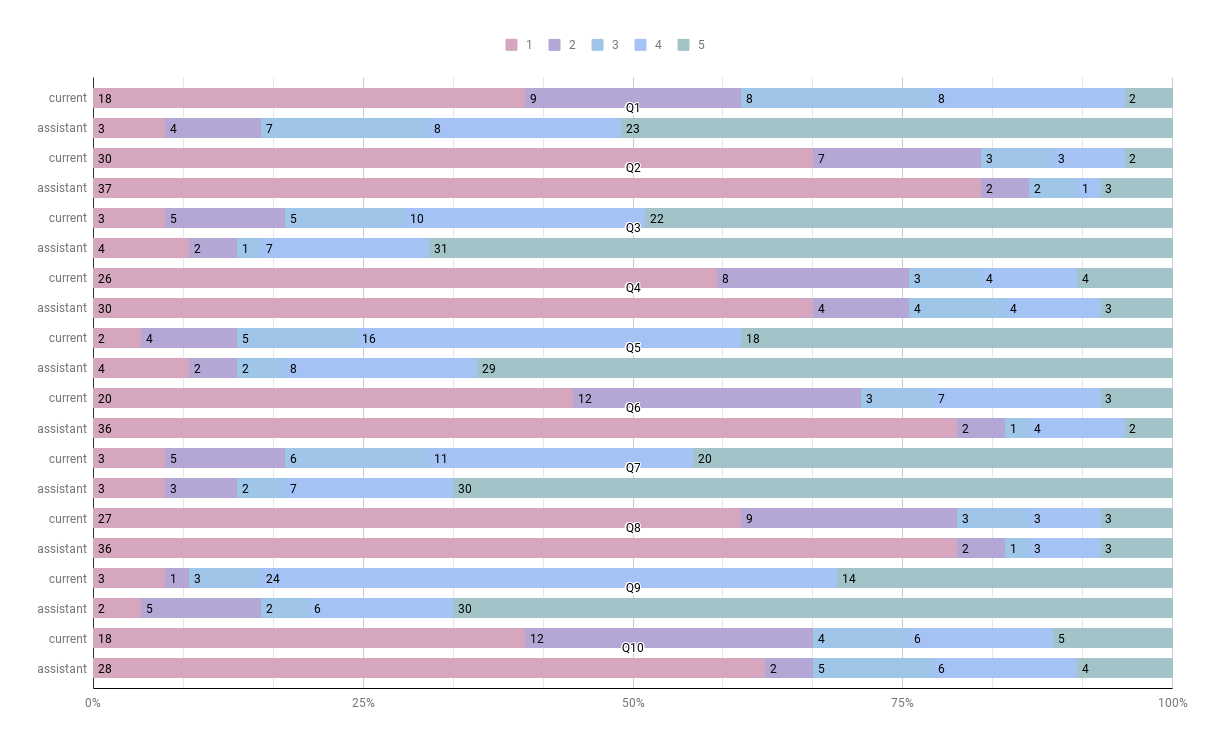
\includegraphics[width=\columnwidth]{images/fig109}
\caption{Results of SUS scores between {\it current} (Clinician-Only) and {\it assistant} (Clinician-AI) conditions. The bars represent the mean score for each question, {\it i.e.}, ranging from 1 = ``Strongly disagree'' to 5 = ``Strongly agree'' of the scale. The SUS questionnaire consists of ten questions (Q1 to Q10), displaying the results of each question in two rows of {\it current} and {\it assistant} conditions. A visual representation provides information on participants' responses to each question, allowing for comparative analysis.}
\label{fig:fig109}
\end{figure}
%%%%%%%%%%%%%%%%%%%%%%%%%%%%%%%%%%%%%%%%%%%%%%%%%%%

The \ac{NASA-TLX} questionnaire was used to measure {\it workload}, leading us to understand the cognitive load change between conditions.
From these results, the statistical analysis showed a significant impact (p = 0.03 $<$ 0.05) when comparing both conditions for the {\it workload} measurements.
More precisely, the results indicated that the Clinician-AI (F = 0.819) condition perceived a lower workload (which is better) compared to the Clinician-Only (F = 5.729) condition.
Our findings showed a reduced workload compared to the baseline scenario, indicating that the Clinician-AI condition effectively supported clinicians in their diagnostic tasks.
Specifically, the results showed that the Clinician-AI condition was associated with lower perceived mental and physical demands (Section~\ref{sec:app003004003} of Appendix~\ref{chap:app003}) compared to the condition without the \ac{AI} technique.
On the other hand, performance (Section~\ref{sec:app003004004} of Appendix~\ref{chap:app003}) was perceived negatively on the Clinician-AI condition.
This may occur due to the increasing number of visualization modalities, and higher information to be analyzed ({\it e.g.}, explanations provided by the assistant).
However, these findings indicate that the \ac{AI} assistant reduces clinicians' cognitive and physiological demands during medical decision-making tasks.
Clinicians reported lower demands with higher perceived efficiency and performance, indicating that the \ac{AI} assistance system alleviated cognitive load and enhanced their efficiency in radiology workflows.

To understand the perceived usefulness of the \ac{AI} assistance, we conducted qualitative {\it post-task} interviews and {\it open-ended} questions (Section~\ref{sec:app003005002} of Appendix~\ref{chap:app003}) to gather clinicians' perspectives on the system's value and practicality in their daily practice.
Qualitative analysis indicated clinicians' high acceptance of the \ac{AI} assistant.
Most clinicians (41/45) accepted the \ac{AI} algorithm in their daily work.
They recognized the potential of \ac{AI} to improve their performance and workflow (28/45).
Comments highlighted the valuable role of the assistant in enhancing diagnostic accuracy, reducing workload, and enabling new quantitative information to be added to reports: ``The system [{\it BreastScreening-AI}] will be a great asset for us'' (C6).
Indeed, clinicians (33/45) expressed positive views on the system's ability to improve diagnostic accuracy, provide timely and relevant information, and facilitate more informed decision-making.
The results indicated that design interventions played a crucial role in enhancing the perceived usefulness of the system.
Integrating \ac{AI} technologies in radiology was seen as a promising approach to augment clinical practices and enable better patient care.

In conclusion, integrating an intelligent agent into the clinical workflow was well-received by clinicians.
This success is due to strategic design interventions, informed by a human-centered approach, providing substantial insights for our {\bf RQ5.1}.
The \ac{AI} assistant received favorable feedback from clinicians, resulting in higher levels of acceptance, satisfaction, and usability when compared to the Clinician-Only scenario.
Notably, the \ac{AI} assistant effectively reduced workload, while also being perceived as valuable in enhancing diagnostic accuracy and improving overall clinical practices.
These findings underscore the potential of \ac{AI}-assisted techniques in optimizing the radiology workflow and empowering clinicians to make well-informed decisions.
The positive reception and acceptance of the \ac{AI} assistant by clinicians highlight the importance of integrating intelligent agents into medical practices, paving the way for continued advancements in healthcare delivery.
As \ac{AI} technologies continue to evolve and improve, it is crucial to foster ongoing collaboration between clinicians, researchers, and technology developers to ensure the responsible and ethical integration of \ac{AI} in radiology and beyond.
By harnessing the full potential of \ac{AI}-assisted techniques, we can aspire to achieve higher levels of precision, productivity, and quality in healthcare, ultimately benefitting both medical professionals and the patients they serve.

\subsection{RQ5.2: Understanding and Trust Enhancement}
\label{sec:chap005006002}

To address the research question {\bf RQ5.2}, we investigated how design techniques can improve clinicians' understanding and trust of the \ac{AI} recommendations by considering the explainability power of the system (Figure~\ref{fig:fig111}).
We measured clinicians' understating, while assessing clinicians' trust across the Model of Trust~\cite{CALISTO2021102607} using the \ac{DOTS} questionnaire (Section~\ref{sec:app003004007} of Appendix~\ref{chap:app003}) for this purpose.
In addition, we collected feedback (Section~\ref{sec:app003005002} of Appendix~\ref{chap:app003}) on the explainability functionalities of the system through qualitative interviews so that we can understand how well the system provides explanations for its \ac{AI} recommendations.

%%%%%%%%%%%%%%%%%%%%%%%%%%%%%%%%%%%%%%%%%%%%%%%%%%%
\begin{figure}[htbp]
\centering
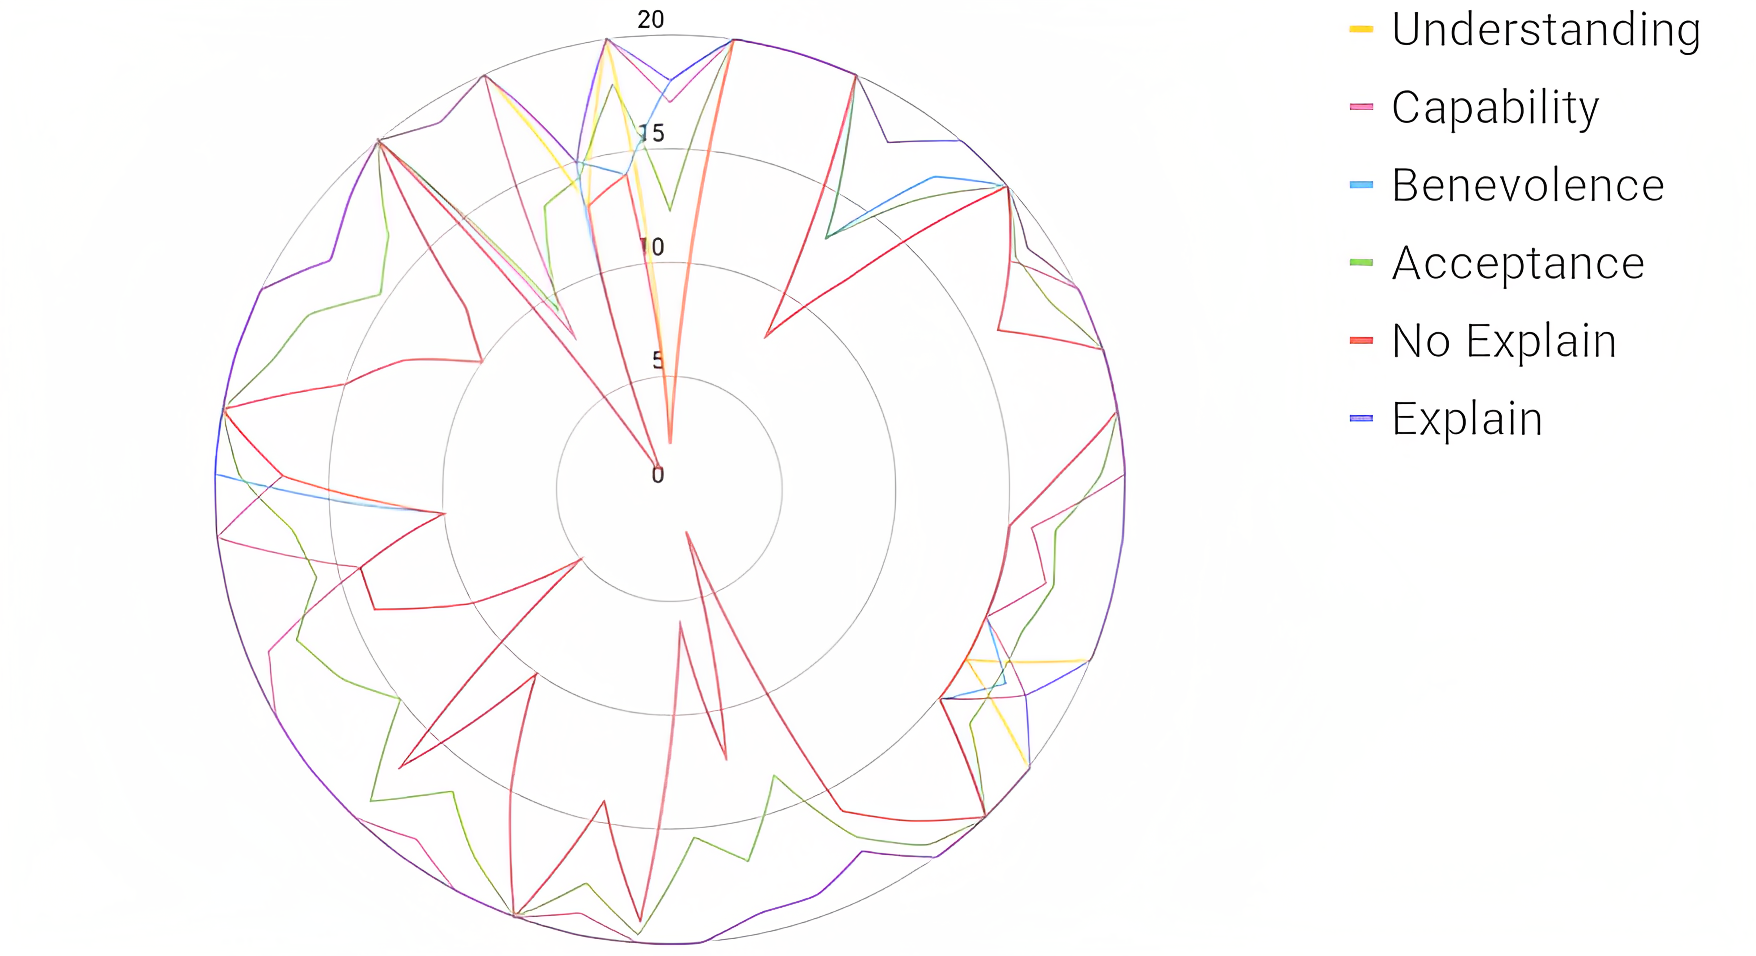
\includegraphics[width=\columnwidth]{images/fig111}
\caption{Results of DOTS and acceptance scores for the {\it assistant} (Clinician-AI) conditions. Each question is ranging from 1 = ``Strongly disagree'' to 20 = ``Strongly agree'' of the scale. The figure provides a visual representation of the participant's responses to perceived {\it Understanding}, {\it Capability}, and {\it Benevolence} of the DOTS scores. Additionally, we measured perceived overall {\it Acceptance} on the assistant, as well as differences in acceptance when clinicians do not ask ({\it No Explain}) or ask ({\it Explain}) for explanations.}
\label{fig:fig111}
\end{figure}
%%%%%%%%%%%%%%%%%%%%%%%%%%%%%%%%%%%%%%%%%%%%%%%%%%%

In this study, we employed a visual information technique utilizing heatmaps to highlight regions of severity in the recommendations of the \ac{AI} system.
The heatmap information visualization effectively conveyed the severity of lesions, with hotter colors (Figure~\ref{fig:fig032}) indicating higher severity.
The results from the \ac{DOTS} questionnaire (Figure~\ref{fig:fig111}) indicated that 98\% of the clinicians comprehended the reasoning behind the system, demonstrating a high level of understanding.
Specifically, clinicians exhibited greater levels of perceived understanding when actively engaging with the assistant by pressing the {\it Explain} button (M = 19.7, SD = 2.92) compared to refraining from pressing it (M = 10, SD = 7).
Furthermore, 93\% of the clinicians expressed trust in the system's capabilities, providing evidence of their confidence in the \ac{AI} recommendations for accurate patient diagnosis.
Through the introduction of {\it 6.1. Accept}, {\it 6.3. Reject}, and {\it 6.2. Explain} buttons (Figure~\ref{fig:fig040}), perceived benevolence (M = 14.67, SD = 5.24) was increased while providing control and flexibility of the final diagnosis.
After asking for an explanation, 76\% of the clinicians increased their agreement ({\it i.e.}, pressing the {\it Accept} button) with the final diagnostic.

Finally, 91\% accept and prefer the \ac{AI} setup (Figure~\ref{fig:fig111}).
Trust values in our assistant (M = 18.81, SD = 2.96) were significantly higher (p = 0.0003 $<$ 0.05) when compared to clinicians who did not press the {\it Explain} button (M = 12.43, SD = 3.21).
Bringing higher levels of acceptance to the \ac{AI} recommendations of the assistant when explaining the severity classification of lesions through heatmaps.
Additionally, there was no significant imbalance in prior frequency for using the {\it BreastScreening-AI} framework.

In conclusion, our study addressed the research question {\bf RQ5.2} by investigating how design techniques can enhance clinicians' understanding and trust in \ac{AI} recommendations, considering the explainability power of the system.
We employed various metrics and questionnaires to assess clinicians' understanding and trust.
Using heatmaps as a visual information technique effectively conveyed the severity of lesions, and clinicians exhibited a high level of understanding, comprehending the reasoning behind the system.
This resulted in higher levels of perceived understanding, where clinicians expressed increased trust in the system's capabilities.
The inclusion of control functionalities further increased perceived benevolence.
Moreover, clinicians preferred the \ac{AI} setup, indicating a positive acceptance of the \ac{AI} recommendations.
Our findings demonstrate that the explainability functionalities achieved through our design process enhance clinicians' understanding and trust in autonomous recommendations, promoting their acceptance and preference for the \ac{AI} setup.

\subsection{RQ5.3: Workflow Impact}
\label{sec:chap005006003}

In this section, we present the results obtained to answer research question {\bf RQ5.3}, which focuses on the impact of \ac{AI} assistance on the medical workflow, including accuracy (Section~\ref{sec:app003004009003} of Appendix~\ref{chap:app003}), time performance (Section~\ref{sec:app003004009}), and variability (Section~\ref{sec:app003004008}) in patient classification.
We begin by investigating the rates of \acp{FP} and \acp{FN} with and without \ac{AI} assistance.
Then, we examine the diagnostic time and breast severity concerning using \ac{AI} assistance.
Next, we delve into the clinical impact of \ac{AI} assistance, exploring the improvement in accuracy and time performance.
Lastly, we discuss the alterations in clinical workflows resulting from integrating \ac{AI} assistance.
By presenting these results, we aim to provide a comprehensive understanding of the \ac{AI} assistance impact on the medical workflow.
The findings shed light on the benefits of \ac{AI} in healthcare settings, including enhanced accuracy, reduced diagnostic time, and improved consistency in patient classification.

The rates of \acp{FP} and \acp{FN} (Table~\ref{tab:tab017}) were compared between the Clinician-Only and the Clinician-AI conditions (Section~\ref{sec:app003004009001} of Appendix~\ref{chap:app003}).
The results demonstrated a reduction in \acp{FP} with \ac{AI} assistance, resulting in fewer cases where radiologists provided a higher severity classification than the actual severity.
Specifically, the \ac{FP} rates decreased from 39\% in the Clinician-Only to 15\% in the Clinician-AI conditions.
This indicates a significant reduction in situations where radiologists provided a higher severity classification (\ac{BI-RADS}) than the actual severity.
The reduction in \acp{FP} by 24\% highlights the effectiveness of \ac{AI} assistance in improving the accuracy of the patient classification and reducing the occurrence of unnecessary procedures or treatments~\cite{10.1001/jamainternmed.2014.981}.
Additionally, the rates of \acp{FN} were reduced by 19\% change when \ac{AI} assistance was utilized.
This indicates that \ac{AI} assistance improved the detection and classification of breast abnormalities, leading to a more accurate diagnosis and reducing the chances of missing critical cases.
These findings highlight the potential of AI assistance in improving patient classification accuracy and reducing \acp{FP} and \acp{FN}.

%%%%%%%%%%%%%%%%%%%%%%%%%%%%%%%%%%%%%%%%%%%%%%%%%%%
% Please add the following required packages to your document preamble:
% \usepackage{multirow}
% \usepackage{graphicx}
\begin{table}[]
\resizebox{\textwidth}{!}{%
\begin{tabular}{|c|cc|cccc|cccc|}
\hline
\multirow{3}{*}{Groups} &
  \multicolumn{2}{c|}{Low} &
  \multicolumn{4}{c|}{Medium} &
  \multicolumn{4}{c|}{High} \\ \cline{2-11} 
 &
  \multicolumn{1}{c|}{Cli.-Only} &
  Cli.-AI &
  \multicolumn{1}{c|}{Cli.-Only} &
  \multicolumn{1}{c|}{Cli.-AI} &
  \multicolumn{1}{c|}{Cli.-Only} &
  Cli.-AI &
  \multicolumn{1}{c|}{Cli.-Only} &
  \multicolumn{1}{c|}{Cli.-AI} &
  \multicolumn{1}{c|}{Cli.-Only} &
  Cli.-AI \\ \cline{2-11} 
 &
  \multicolumn{1}{c|}{FPs} &
  FPs &
  \multicolumn{1}{c|}{FPs} &
  \multicolumn{1}{c|}{FPs} &
  \multicolumn{1}{c|}{FNs} &
  FNs &
  \multicolumn{1}{c|}{FPs} &
  \multicolumn{1}{c|}{FPs} &
  \multicolumn{1}{c|}{FNs} &
  FNs \\ \hline
Intern &
  \multicolumn{1}{c|}{0.58} &
  0.42 &
  \multicolumn{1}{c|}{0.75} &
  \multicolumn{1}{c|}{0.08} &
  \multicolumn{1}{c|}{0.08} &
  0.08 &
  \multicolumn{1}{c|}{0.33} &
  \multicolumn{1}{c|}{0.08} &
  \multicolumn{1}{c|}{0.17} &
  0.08 \\ \hline
Junior &
  \multicolumn{1}{c|}{0.63} &
  0.13 &
  \multicolumn{1}{c|}{0.38} &
  \multicolumn{1}{c|}{0.13} &
  \multicolumn{1}{c|}{0.13} &
  0.13 &
  \multicolumn{1}{c|}{0.50} &
  \multicolumn{1}{c|}{0.25} &
  \multicolumn{1}{c|}{0.13} &
  0.13 \\ \hline
Middle &
  \multicolumn{1}{c|}{0.43} &
  0.21 &
  \multicolumn{1}{c|}{0.79} &
  \multicolumn{1}{c|}{0.21} &
  \multicolumn{1}{c|}{0.07} &
  0.07 &
  \multicolumn{1}{c|}{0.21} &
  \multicolumn{1}{c|}{0.07} &
  \multicolumn{1}{c|}{0.14} &
  0.07 \\ \hline
Senior &
  \multicolumn{1}{c|}{0.45} &
  0.36 &
  \multicolumn{1}{c|}{0.73} &
  \multicolumn{1}{c|}{0.09} &
  \multicolumn{1}{c|}{0.09} &
  0.18 &
  \multicolumn{1}{c|}{0.09} &
  \multicolumn{1}{c|}{0.09} &
  \multicolumn{1}{c|}{0.09} &
  0.09 \\ \hline
\end{tabular}%
}
\caption{Comparison of FP and FN rates between the Clinician-Only ({\it Cli.-Only}) setup and the Clinician-AI ({\it Cli-AI}) setup, categorized by severity levels ({\it i.e.}, {\it Low}, {\it Medium}, and {\it High}), across different levels of medical professional experience ({\it i.e.}, {\it Inter}, {\it Junior}, {\it Middle}, and {\it Senior} levels) of clinicians. The table presents the rates of FPs and FNs, providing insights into the performance of the two setups across severity categories and clinician experience levels. For {\it Low} severities (BI-RADS = 1), we only provide FPs rates since we did not consider lower (BI-RADS = 0) rates.}
\label{tab:tab017}
\end{table}
%%%%%%%%%%%%%%%%%%%%%%%%%%%%%%%%%%%%%%%%%%%%%%%%%%%

From a dataset of 289 patients, we analyzed our results to explore the relationship between diagnostic time and breast severity (Section~\ref{sec:app003004005} of Appendix~\ref{chap:app003}).
Our findings revealed notable differences in diagnostic time across different severity levels.
For patients with low severity ({\bf P1}), the average diagnostic time in the Clinician-Only condition was 146 seconds (SD = 86.17), whereas the Clinician-AI condition showed a shorter average of 89 seconds (SD = 74.13).
Similarly, for patients with medium severity ({\bf P2}), the Clinician-Only condition had an average diagnostic time of 78 seconds (SD = 48.05), while the Clinician-AI condition exhibited a slightly lower average of 77 seconds (SD = 96.80).
Notably, patients with high severity ({\bf P3}) experienced a longer average diagnostic time of 116 seconds (SD = 65.70) in the Clinician-Only condition compared to the Clinician-AI condition, which had an average of 64 seconds (SD = 86.94).
Furthermore, the \ac{ANOVA} statistical test revealed a significant effect of clinical experience groups on diagnostic time for severity cases between conditions (F = 3.25, p = 0.03 $<$ 0.05).
These findings demonstrate that \ac{AI} assistance significantly reduces diagnostic time across different severity levels.
Moreover, the analysis highlights the influence of clinicians' time performance with different medical professional experiences in the decision-making process of diagnosing patients.

The introduction of \ac{AI} assistance positively influenced both inter-variability and intra-variability agreement (Section~\ref{sec:app003004008} of Appendix~\ref{chap:app003}) among clinicians during patient classification.
With \ac{AI} assistance, there were significant reductions in variability.
Regarding inter-variability, the \ac{CV} decreased from 57.69\% to 46.69\% for patients with low severity, demonstrating improved agreement and consistency among clinicians.
For patients with a medium severity, inter-variability improved by 3.28\%, while the most notable improvement of 34.10\% was observed for patients with high severity.
Intra-variability also decreased within specific clinician groups, including interns, juniors, middles, and seniors, with reductions ranging from 6.65\% to 23.66\%.
These findings indicate that \ac{AI} assistance enhances inter-variability agreement and reduces variability within clinician groups based on their medical professional experience.
Overall, \ac{AI} assistance promotes more reliable and consistent patient classification outcomes, improving diagnostic decisions.
Therefore, clinicians benefit from improved agreement and enhanced diagnosis consistency, improving patient care.

In summary, the results of this study demonstrate the positive impact of \ac{AI} assistance on the medical workflow.
The utilization of \ac{AI} assistance significantly improves accuracy in patient classification, reduces the time required for various tasks, and enhances inter-rater agreement.
These findings support the integration of \ac{AI} technologies in healthcare settings, emphasizing their potential to enhance efficiency, accuracy, and consistency in decision-making during breast cancer diagnosis.

\subsection{Summary}
\label{sec:chap005006004}

Here, we encapsulate the main findings of our study.
These results summarize each facet of our investigation, elucidating the impact of \ac{AI} medical assistance and the advantages of employing a human-centered design approach.
By analyzing these crucial aspects, we aim to elucidate the effects of design interventions on clinicians' experiences and perceptions.
The analysis of satisfaction and acceptance encompasses usability, workload, and usefulness, while understanding and trust enhancement focuses on clinicians' comprehension and confidence in \ac{AI} recommendations.
Finally, the investigation of workflow impact delves into accuracy, diagnostic time, and variability in patient classification.

In terms of satisfaction and acceptance ({\bf RQ5.1}), our results showed that the introduction of \ac{AI} assistance through design interventions significantly improved clinicians' satisfaction and acceptance of \ac{AI} assistance in radiology.
The \ac{SUS} questionnaire results indicated that the \ac{AI}-assisted condition received 69\% higher agreement, demonstrating a 91\% higher usefulness of the \ac{AI}-assisted techniques compared to the Clinician-Only.
In fact, 82\% of clinicians reported positive perceptions of the system's usability, ease of use, and integration with workflow.
These findings highlight the effectiveness of design interventions in enhancing clinicians' satisfaction and acceptance of \ac{AI} assistance in radiology.

Regarding understanding and trust enhancement ({\bf RQ5.2}), our study revealed that design techniques could improve clinicians' understanding and trust in \ac{AI} recommendations.
About 85\% of clinicians exhibited a high level of understanding and trust in the system's capabilities.
Including explainability functionalities, such as heatmaps and control functionalities, increased perceived understanding and benevolence, respectively.
Specifically, 62\% of clinicians positively accepted the \ac{AI} setup, indicating their preference for \ac{AI} recommendations.
These findings emphasize the importance of explainability in enhancing clinicians' understanding and trust in \ac{AI} assistance.

Regarding workflow impact ({\bf RQ5.3}), our results demonstrated that \ac{AI} assistance positively impacts the medical workflow in radiology.
Using \ac{AI} assistance reduced the medical error percentile by 15\% for \acp{FP} and 2\% for \acp{FN}, improving patient classification accuracy.
Diagnostic time was significantly reduced by an average of 50 seconds per patient across different severity levels, indicating enhanced efficiency.
Furthermore, \ac{AI} assistance improved clinician agreement and consistency, reducing inter-variability and intra-variability.
These findings highlight the potential of \ac{AI} assistance to optimize the medical workflow, leading to better patient care and treatment decisions.

In conclusion, our work explored several aspects of clinician interactions with \ac{AI} assistance in radiology, including satisfaction, acceptance, understanding, trust, and workflow transformation.
By employing a human-centered approach and design interventions, our findings underscore the success of integrating intelligent agents into real-world clinical settings.
These interventions have boosted user satisfaction and trust in \ac{AI} recommendations, enhancing clinicians' understanding.
Including intelligent agents has optimized the medical workflow, enhancing diagnostic accuracy, reducing diagnostic time, and improving consistency, thereby strengthening decision-making reliability and clinicians' efficiency.

\section{Discussion}
\label{sec:chap005007}

In this section, we summarize the study's findings, discuss their implications, and identify areas for further investigation.
We contextualize our findings within the existing research landscape, compare them with previous studies, and highlight their practical significance.
We also acknowledge the limitations of the study and propose future directions.
Further discussion are provided in Section~\ref{sec:app003005} of Appendix~\ref{chap:app003}.

\subsection{Findings}
\label{sec:chap005007001}

Interpreting the results in light of existing literature~\cite{10.1145/3411764.3445432} and theoretical frameworks~\cite{10.1145/3311957.3361858} allows us to contextualize our findings within the broader research landscape and theoretical understanding of the topic.
It provides an opportunity to compare and contrast our results with previous studies~\cite{CALISTO2022102285, CALISTO2021102607}, identify areas of alignment or divergence, and discuss the practical significance of our findings.
Additionally, addressing the study's limitations and suggesting areas for further investigation helps to acknowledge the scope of our work and identify avenues for future research (Section~\ref{sec:app003005004}).
Our study examined various elements of clinician interactions with \ac{AI} assistance in radiology.
Using a human-centered approach and design interventions, we successfully integrated intelligent agents into clinical settings.
The research revealed significant results and new insights into the practical advantages of medical \ac{AI} assistance.

Starting with satisfaction and acceptance ({\bf RQ5.1}), our findings highlight the crucial role of integrating \ac{HCI} principles into the design process of \ac{AI} systems.
Through these design interventions, we were able to notably enhance the levels of satisfaction and acceptance among clinicians toward the final solution.
Our results align with prior studies~\cite{10.1145/3411764.3445432}, emphasizing the benefits of design interventions and reinforcing the essential role of \ac{HCI} principles in promoting positive \ac{AI} system engagement.
The higher agreement percentages and positive perceptions of usability, ease of use, and workflow integration highlight the effectiveness of design interventions in enhancing clinicians' satisfaction and acceptance of \ac{AI} assistance (Section~\ref{sec:app003005002} of Appendix~\ref{chap:app003}).
By considering \ac{HCI} principles, such as \ac{UCD} and usability testing, in the development of \ac{AI} systems, we can ensure that the design interventions effectively address clinicians' needs and preferences, leading to improved user satisfaction and acceptance.

In terms of understanding and trust enhancement ({\bf RQ5.2}), our study demonstrated the effectiveness of design techniques in improving clinicians' understanding and trust in \ac{AI} recommendations.
The results align with theoretical frameworks~\cite{10.1145/3311957.3361858} that emphasize the significance of explainability and transparency in fostering trust in \ac{AI} systems.
By incorporating explainability functionalities, such as heatmaps and control functionalities, we observed improvements in clinicians' understanding and perceived benevolence of the \ac{AI} system.
These enhancements contributed to their acceptance and preference for \ac{AI} recommendations.
The findings highlight the importance of incorporating explainability features in \ac{AI} system design to promote understanding and trust among clinicians.

Regarding workflow impact ({\bf RQ5.3}), our results indicated that \ac{AI} assistance positively impacts the medical workflow in radiology (Section~\ref{sec:app003005001} of Appendix~\ref{chap:app003}).
The reduction in \acp{FP} and \acp{FN}, improved accuracy in patient classification, and reduced diagnostic time highlight the potential of \ac{AI} assistance to optimize the medical workflow and enhance patient care.
These findings align with previous studies demonstrating the benefits of \ac{AI} in improving diagnostic accuracy and efficiency in healthcare settings.
The enhanced inter-rater agreement and reduced variability further support the notion that \ac{AI} assistance promotes more consistent and reliable patient classification outcomes.

In this study, we explored how design interventions could guide us in developing an optimal solution for radiology (Section~\ref{sec:app003006}), thereby underscoring the pivotal role of \ac{HCI} principles in designing \ac{AI} systems.
Our findings reveal the transformative potential of design interventions in augmenting decision-making and boosting diagnostic efficiency.
The outcomes underscore the necessity of considering \ac{HCI} principles and optimizing workflow integration when introducing \ac{AI} systems into healthcare environments.
We advocate for embracing \ac{HCI} principles in the design process to develop \ac{AI} systems that cater more effectively to clinicians' needs, ultimately enhancing diagnostic performance.

\subsection{Design Implications}
\label{sec:chap005007002}

Our findings highlight the potential of \ac{AI} assistance to enhance clinicians' decision-making, efficiency, and patient care in radiology.
The effective execution of design interventions and \ac{HCI} principles is crucial for achieving optimal solutions, resulting in enhanced user satisfaction, acceptance, understanding, and trust.
Applying \ac{HCI} principles and strategic design interventions is vital for successful \ac{AI} incorporation in clinical practice.
Enhancing clinicians' satisfaction and acceptance enables more effective utilization of \ac{AI} technologies in healthcare settings.
Design techniques that promote understanding and trust in \ac{AI} recommendations empower clinicians to make informed decisions, leading to better patient care outcomes.
Workflow improvements, including reduced diagnostic time, increased accuracy, and enhanced consistency, have significant implications for clinical practice, potentially improving the efficiency and effectiveness of diagnoses.
Optimizing the medical workflow through \ac{AI} assistance ultimately improves patient outcomes and enhances the overall quality of healthcare delivery.

\noindent
Based on our findings, we propose the following design implications:

\vspace{0.05mm}

\begin{itemize}

\item \textbf{Workflow Understanding and Task-Specific Evaluations}:
Researchers should aim to develop \ac{AI} systems tailored to the specific characteristics of clinical workflows and the straightforward tasks of clinicians.
This understanding is essential for recognizing clinicians' requirements and designing intelligent agents that effectively support their decision-making processes.
When evaluating the performance of \ac{AI} systems, it is vital to consider the high-level workflow actions and diagnostic mechanisms to ensure that the evaluations are task agnostic and provide comprehensive insights.

\vspace{0.025mm}

\item \textbf{Concrete Evidence and Insights}:
Intelligent agents should provide clinicians with concrete empirical evidence and insights, highlighting the consequences or benefits of heeding or disregarding different types of \ac{AI} predictions to mitigate diagnostic errors.
This can help address model ambiguity and build trust in the \ac{AI} system.
Researchers can enhance clinicians' understanding of the system's capabilities and limitations by detailing the areas in the \ac{AI} reasoning where mistakes occur and the potential impact on patients.
Providing transparent explanations and granular insights will empower clinicians to make well-informed decisions based on the \ac{AI} outputs.

\vspace{0.025mm}

\item \textbf{Optimizing Precision and Recall with Uncertainty and Explanations}:
When designing \ac{AI} systems, consider optimizing precision and recall metrics while incorporating model uncertainty and explanations.
By optimizing precision and recall, designers can strike a balance between minimizing \acp{FP} and \acp{FN} in the \ac{AI} outputs.
Additionally, providing clinicians with explanations and insights into model uncertainty and misunderstandings can help them better interpret and utilize the \ac{AI} system's recommendations.
This approach ensures clinicians know potential misunderstandings and can make informed decisions based on the system's outputs.

\end{itemize}

\vspace{0.05mm}

These design implications underscore the importance of incorporating principles from the \ac{HCI} community when designing \ac{AI} systems for clinical settings.
Researchers can develop \ac{AI} systems that align with clinicians' needs and preferences by considering the clinical workflow, providing concrete evidence and insights, as well as optimizing precision and recall with uncertainty and explanations.
These implications contribute to the effective integration of \ac{AI} technologies in clinical settings and enhance the overall quality of patient care.
They highlight the valuable contributions of the \ac{HCI} community in guiding the design of \ac{AI} systems that are transparent and supportive of clinicians' decision-making processes.

\subsection{Design Recommendations}
\label{sec:chap005007003}

We provide the following design recommendations to optimize workflow integration, ensuring effective development and implementation of \ac{AI} systems in clinical settings.
These recommendations foster continuous evaluation and improvement by using \ac{HCI} principles.
By following these recommendations, designers can create user-centric \ac{AI} systems that enhance the overall quality of healthcare delivery.

\noindent
Based on our findings, we propose the following design recommendations for incorporating \ac{AI} assistance into radiology practice:

\vspace{0.025mm}

\begin{enumerate}

\item \textbf{Usability}:
Apply user-centered design principles and conduct extensive usability testing involving clinicians to ensure intuitive and seamlessly integrated \ac{AI} systems that enhance user satisfaction and acceptance.

\vspace{0.025mm}

\item \textbf{Explainability and Transparency}:
Incorporate explainability functionalities, such as visualizations and control functionalities, to enhance clinicians' understanding and trust in \ac{AI} recommendations, fostering transparency and interpretability.

\vspace{0.025mm}

\item \textbf{Integration and Workflow Optimization}:
Seamlessly integrate \ac{AI} systems into the clinical workflow, optimizing compatibility, performance, and efficiency to reduce diagnostic time and improve productivity.

\vspace{0.05mm}

\item \textbf{Longitudinal Studies and Continuous Evaluation}:
Conduct longitudinal studies, gather feedback, and iterate on the design based on evolving needs and challenges, ensuring the long-term effectiveness and alignment of \ac{AI} systems with clinical practice.

\end{enumerate}

\vspace{0.05mm}

By incorporating these design recommendations into the development and implementation of \ac{AI} assistance systems, we can enhance user satisfaction, acceptance, understanding, trust, and workflow optimization in radiology practice.
These recommendations promote the effective integration of \ac{AI} technologies into clinical workflows (Section~\ref{sec:app003005003}), ultimately improving patient care and outcomes.

\subsection{Limitations}
\label{sec:chap005007004}

While our study provides valuable insights, it is essential to acknowledge its limitations.
One limitation is the specific focus on radiology, which may limit the generalizability of the findings to other medical domains.
Future research should explore the applicability and effectiveness of design interventions in different medical domains to gain a more comprehensive understanding of the impact of \ac{AI} assistance.

Further investigations should also consider longitudinal studies to examine \ac{AI} assistance's long-term effects and sustainability in clinical practice.
Understanding the evolving dynamics of clinician-\ac{AI} interaction over time and capturing potential challenges or benefits that emerge in the real-world deployment of \ac{AI} assistance would provide valuable insights for successfully integrating \ac{AI} technologies into routine healthcare practice.
Additionally, it is crucial to continue exploring the ethical and social implications of \ac{AI} assistance in radiology and healthcare in general.
This includes examining the impact on the roles and responsibilities of healthcare professionals, trust and acceptance, privacy and security considerations, and the potential biases or disparities that may arise in using \ac{AI} algorithms.

\section{Conclusion}
\label{sec:chap005008}

Integrating \ac{AI} techniques into the clinical workflow, along with design interventions, presents promising opportunities in healthcare.
The effective execution of design interventions and applying \ac{HCI} principles are crucial for achieving optimal solutions, leading to enhanced user satisfaction, acceptance, understanding, and trust.
By interpreting our results in the context of existing literature and theoretical frameworks, we have gained valuable insights into the practical implications of \ac{AI} assistance in radiology, underscoring the significance of incorporating \ac{HCI} principles in designing \ac{AI} systems.
The consolidation of \ac{HCI} principles and strategic design interventions is vital for successfully integrating \ac{AI} into clinical practice, playing a crucial role in achieving optimal solutions and enhancing diagnostic performance.

When considering \ac{HCI} principles such as user-centered design and usability testing, designers can create \ac{AI} systems that effectively address clinicians' needs and preferences, leading to improved user satisfaction and acceptance.
Furthermore, the study demonstrates the effectiveness of design techniques in enhancing clinicians' understanding and trust in \ac{AI} recommendations.
Incorporating explainability functionalities, such as heatmap visualizations and control mechanisms, improve clinicians' understanding of the system's reasoning and fosters trust in \ac{AI} recommendations.
This finding aligns with theoretical frameworks emphasizing transparency and explainability in building trust in \ac{AI} systems.

The workflow impact of \ac{AI} assistance is also evident from the results.
The reduction in \acp{FP} and \acp{FN}, improved accuracy in patient classification, and reduced diagnostic time indicate the potential of \ac{AI} assistance to optimize the medical workflow and enhance patient care.
These findings align with previous research demonstrating the benefits of \ac{AI} in improving diagnostic accuracy and efficiency in healthcare settings.
To optimize workflow integration, ensuring the effective development and implementation of \ac{AI} systems in clinical settings, several design recommendations are proposed.
These recommendations emphasize the importance of usability, explainability, transparency, integration, and continuous evaluation.
By following these recommendations, designers can create user-centric \ac{AI} systems that enhance the overall quality of healthcare delivery.

It is essential to acknowledge the limitations of the study.
The specific focus on radiology may limit the generalizability of the findings to other medical domains.
Future research should explore the applicability and effectiveness of design interventions in different healthcare contexts.
Longitudinal studies are also needed to examine the long-term effects and sustainability of \ac{AI} assistance in clinical practice.

In conclusion, this study highlights the promising opportunities of integrating \ac{AI} techniques into the clinical workflow through design interventions, particularly in radiology.
Our results show that the effective execution of these interventions and applying \ac{HCI} principles are crucial for achieving optimal solutions.
By incorporating \ac{HCI} principles and optimizing workflow integration, \ac{AI} systems can support decision-making and enhance clinicians' efficiency.
The findings provide valuable insights for successfully integrating \ac{AI} technologies into routine healthcare practice.